% VLDB template version of 2020-08-03 enhances the ACM template, version 1.7.0:
% https://www.acm.org/publications/proceedings-template
% The ACM Latex guide provides further information about the ACM template
%!TEX program = pdflatex

\documentclass[sigconf, nonacm, pdfa]{acmart}


\usepackage{balance}
\usepackage{enumitem}

\usepackage{multirow}

\usepackage{graphicx}

\usepackage{microtype}  %处理换行
\usepackage{subcaption} % 需要subcaption宏包支持子图
\usepackage{caption}

\usepackage{array}
%\usepackage[all]{nowidow}
\usepackage{times}

% %% The following content must be adapted for the final version
% % paper-specific
\newcommand\vldbdoi{XX.XX/XXX.XX}
\newcommand\vldbpages{XXX-XXX}
% issue-specific

\newcommand\vldbvolume{19}
\newcommand\vldbissue{2}
\newcommand\vldbyear{2025}
% should be fine as it is
\newcommand\vldbauthors{\authors}
\newcommand\vldbtitle{\shorttitle} 
% leave empty if no availability url should be set
\newcommand\vldbavailabilityurl{https://github.com/zhujx001/Hybrid-ANNS-Experiment}
% whether page numbers should be shown or not, use 'plain' for review versions, 'empty' for camera ready
\newcommand\vldbpagestyle{empty} 

\usepackage[a-2b,mathxmp]{pdfx}



\begin{document}
	%\begin{sloppypar}
	\title{An Experimental Evaluation of Hybrid Querying on Vectors (EA\&B)}
	
	\author{Jiaxu Zhu}
	\affiliation{%
		\institution{Huazhong University of Science and Technology}
	}
	
	\author{Jiayu Yuan}
	\affiliation{%
		\institution{Huazhong University of Science and Technology}
	}
	
	\author{Kaiwen Yang}
	\affiliation{%
		\institution{Huazhong University of Science and Technology}
	}
	
	\author{Xiaobao Chen}
	\affiliation{%
		\institution{Huazhong University of Science and Technology}
	}
	
	\author{Shihuan Yu}
	\affiliation{%
		\institution{Huazhong University of Science and Technology}
	}
	
	\author{Hongchang Lv}
	\affiliation{%
		\institution{Huazhong University of Science and Technology}
	}
	
	\author{Yan Li}
	\affiliation{%
		\institution{Wuhan University of Technology}
	}
	
	\author{Bolong Zheng}
	\affiliation{%
		\institution{Huazhong University of Science and Technology}
	}
	%%
	%% The "author" command and its associated commands are used to define the authors and their affiliations.
	
	
	% \author{Mengzhao Wang$^1$, Xiaoliang Xu$^1$, Qiang Yue$^1$, Yuxiang Wang$^{1,*}$}
	% \affiliation{%
		%  \institution{$^1$Hangzhou Dianzi University, China}
		% }
	% \email{{mzwang,xxl,yq,lsswyx}@hdu.edu.cn}
	% \author{Ben Trovato$^1$, Lars Th{\o}rv{\"a}ld$^2$, Valerie B\'eranger$^3$, J\"org von \"Arbach$^3$, Wang Xiu Ying$^3$, Donald Fauntleroy Duck$^3$}
	
	% \affiliation{%
		%   \institution{1. Institute for Clarity in Documentation, Ireland}
		%   \institution{2. The Th{\o}rv{\"a}ld Group, Iceland}
		%   \institution{3. Inria Paris-Rocquencourt, France}
		% }
	
	% \email{trovato@corporation.com, larst@affiliation.org, vb@rocquencourt.com, jaerbach@uni-tuebingen.edu, firstname.lastname@ecnu.edu.cn, donald@swa.edu}
	
	%
	% The abstract is a short summary of the work to be presented in the
	% article.
	\begin{abstract}
		Recent studies demonstrate the significant practical value of hybrid queries, which integrate vector search with structured filters (e.g., attribute and range filtering) for refined retrieval.
		However, current evaluations lack unified benchmarking standards and systematic assessment methodologies. Existing studies either fail to cover mainstream algorithms or omit systematic comparisons or in-depth analysis on different methods. To address this issue, we design a comprehensive evaluation framework for hybrid queries. Our study introduces 15 hybrid query algorithms and systematically classifies them based on multiple dimensions, such as index organization and filtering strategy, providing a reference for the categorization of hybrid queries. 

In the experiments, we construct standardized attribute and range sets for attribute filtering and range filtering, respectively, enabling a unified comparison of algorithms in terms of index construction efficiency and query performance. Furthermore, we evaluate the robustness of the algorithms across multiple dimensions, including data distributions, platforms, and scalability on a 100-million-scale dataset.
	 Additionally, we conduct an in-depth analysis of the experimental results based on the underlying principles of algorithms. Extensive experimental results reveal the strengths and weaknesses of each algorithm. Based on the findings, we develop a set of practical guidelines for algorithm selection, offering reliable references for different application scenarios. Furthermore, we identify potential directions for improvement to address the current limitations of these algorithms.
		
	\end{abstract}
	
	
	\maketitle
	
	%%% do not modify the following VLDB block %%
	%%% VLDB block start %%%
	\pagestyle{\vldbpagestyle}
	\begingroup\small\noindent\raggedright\textbf{PVLDB Reference Format:}\\
	\vldbauthors. \vldbtitle. PVLDB, \vldbvolume(\vldbissue): \vldbpages, \vldbyear.\\
	\href{https://doi.org/\vldbdoi}{doi:\vldbdoi}
	\endgroup
	\begingroup
	\renewcommand\thefootnote{}\footnote{\noindent
		This work is licensed under the Creative Commons BY-NC-ND 4.0 International License. Visit \url{https://creativecommons.org/licenses/by-nc-nd/4.0/} to view a copy of this license. For any use beyond those covered by this license, obtain permission by emailing \href{mailto:info@vldb.org}{info@vldb.org}. Copyright is held by the owner/author(s). Publication rights licensed to the VLDB Endowment. \\
		\raggedright Proceedings of the VLDB Endowment, Vol. \vldbvolume, No. \vldbissue\ %
		ISSN 2150-8097. \\
		\href{https://doi.org/\vldbdoi}{doi:\vldbdoi} \\
	}\addtocounter{footnote}{-1}\endgroup
	%%% VLDB block end %%%
	
	%%% do not modify the following VLDB block %%
	%%% VLDB block start %%%
	\ifdefempty{\vldbavailabilityurl}{}{
		
		\begingroup\small\noindent\raggedright\textbf{PVLDB Artifact Availability:}\\
		The source code, data, and/or other artifacts have been made available at \url{\vldbavailabilityurl}.
		\endgroup
	}
	%%% VLDB block end %%%
	
	\section{Introduction}
	
	Nearest Neighbor (NN) search \cite{cover1967nearest} aims to find the closest vector in a given space and serves as a fundamental algorithm in vector retrieval, with widespread applications in recommendation systems   and image retrieval \cite{wang2012scalable}.
	However, with the exponential growth of data volume and the increasing dimensionality of vectors \cite{weber1998quantitative}, traditional NN search methods struggle to meet the demands of real-time search. To address this issue, studies turn to more efficient approaches - Approximate NN (ANN) search ~\cite{arya1998optimal,beis1997shape,gionis1999similarity,malkov2018efficient}, which significantly improve search efficiency by constructing effective indexing structures, albeit at the cost of reduced accuracy.
	
	Nevertheless, as application scenarios grow increasingly complex, simple ANN search can no longer satisfy all practical needs. For instance, Figure~\ref{fig:hybrid ANNS} illustrates a case where users on e-commerce platforms search for clothing items by retrieving visually similar products based on an image. Additionally, users may impose further requirements such as price, color, or brand preferences. Such scenarios necessitate a retrieval system capable of simultaneously addressing vector similarity (e.g., product image) and attribute constraints (e.g., brand name) \cite{tian2023approximate}. When the constraint involves a specific attribute value, this problem refers to Attribute Filtering Approximate Nearest Neighbor (AF-ANN) search ~\cite{NHQ,Filtered-diskann}. For example, a user may seek a green piece of clothing. If the constraint involves a range condition, the problem is known as Range Filtering Approximate Nearest Neighbor (RF-ANN) search ~\cite{serf,iRangeGraph}. For instance, filtering clothes priced between 100 and 200. To meet these application demands, hybrid querying techniques \cite{JD-e-commerce, analyticdb} emerge. Hybrid queries integrate vector retrieval with conditional filtering, optimizing their interaction to significantly enhance efficiency and flexibility in complex query scenarios.
	
	\begin{figure*}
		\centering
		\setlength{\abovecaptionskip}{0.15cm}
		\setlength{\belowcaptionskip}{-0.10cm}

		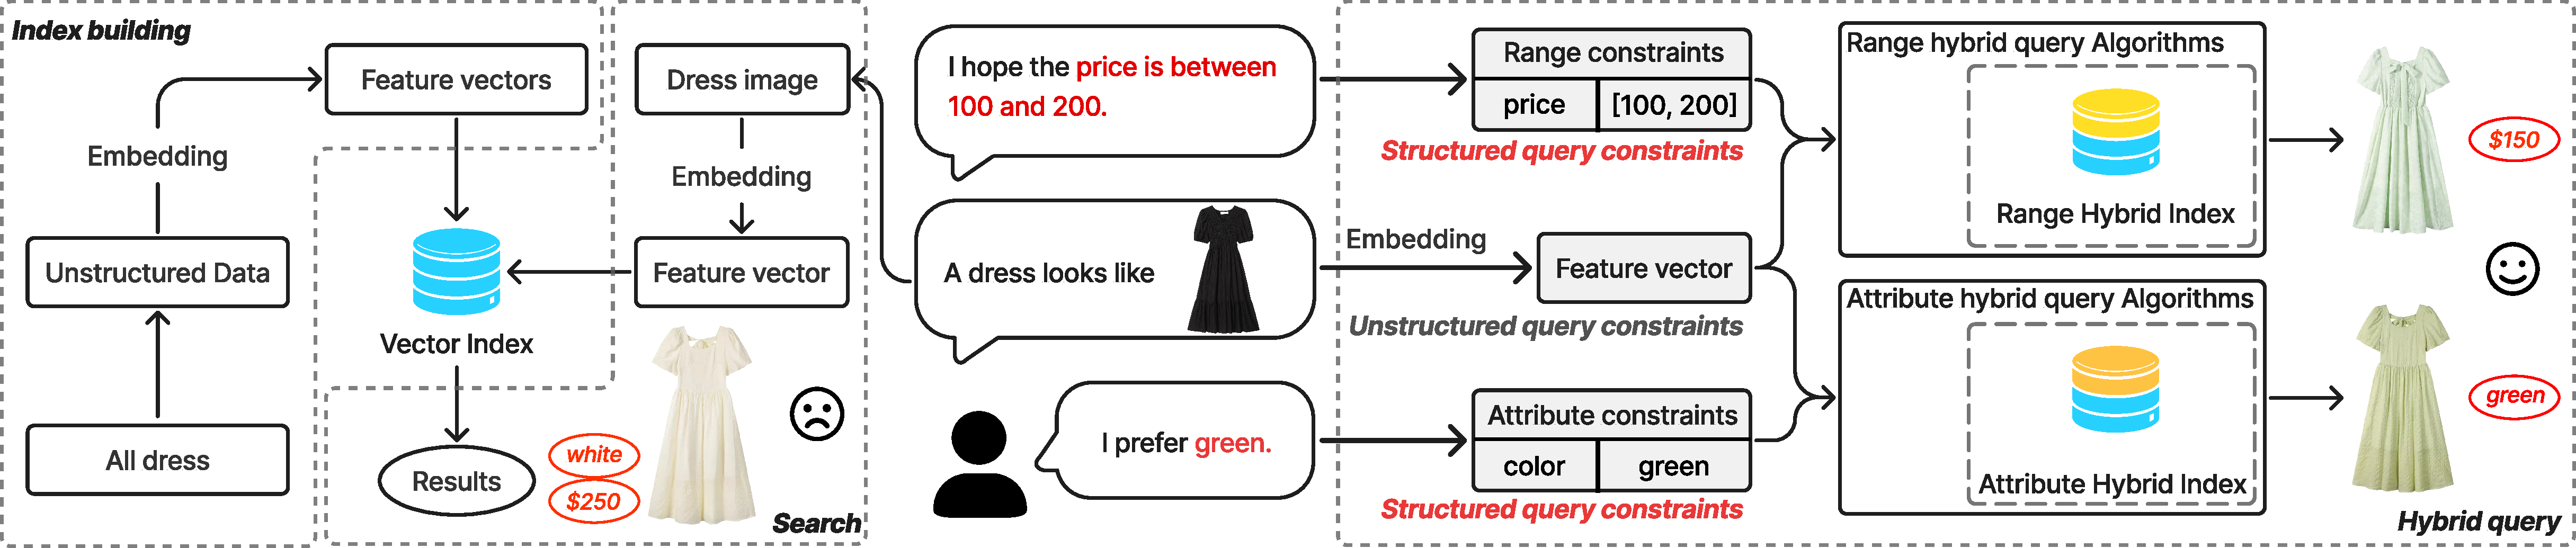
\includegraphics[width=0.92\textwidth]{figures/hybridANNS.pdf}
		\caption{Hybrid Query Example}
		
		\label{fig:hybrid ANNS}
	\end{figure*}
	\subsection{Motivation}
	In recent years, hybrid query algorithms develop rapidly, giving rise to numerous attribute filtering algorithms~\cite{NHQ,diskann} and range filtering algorithms~\cite{serf,iRangeGraph}. In practical applications, the performance of hybrid query algorithms is influenced not only by unstructured data but also closely relates to structured data. For attribute filtering algorithms, factors such as the number of attributes, attribute distribution \cite{UNG}, and attribute selectivity ~\cite{analyticdb,milvus} significantly impact algorithm performance. As for range filtering algorithms, the width of the query range and the characteristics of different datasets play an important role in determining algorithm performance.
	
Although existing studies~\cite{compare,compare2} conduct benchmark evaluations of ANN methods, a systematic experimental study specifically targeting hybrid query algorithms is still lacking. Despite BigANN 2023~\cite{bigann2023} evaluates the performance of some hybrid query algorithms, it still presents the following notable limitations:
	1) The evaluation covers a limited number of algorithms and fails to comprehensively include mainstream methods.
	2) It only uses a single dataset and focuses solely on single-attribute and dual-attribute query scenarios, while not considering the impact of attribute selectivity on query performance.
	3) It only simply compares the query speed and recall of different algorithms, but does not consider key metrics such as the time and space overhead of each algorithm, and it lacks an in-depth analysis of the specific reasons for algorithm performance.
	
To fill this gap, we conduct the first comprehensive experimental evaluation of hybrid query algorithms, systematically analyzing their index construction costs and query efficiency across diverse scenarios. Furthermore, we rigorously assess the robustness of each algorithm under different experimental settings, thereby providing valuable insights for future research and practical applications.
	

	\subsection{Our Contributions}
	
	Our study focuses on the problem of ANN search in hybrid query scenarios and provides a comprehensive review and evaluation of existing algorithms and systems. The main contributions are summarized in the following 5 aspects.
	
	(1)\textbf{ Systematic Classification and Overview.}
	We systematically classify 6 representative attribute filtering algorithms along multiple dimensions, including index organization, filtering strategies, Boolean logic support, and index construction methods. In addition, we survey 5 range filtering algorithms, and provide an overview of one vector library and 3 vector databases. These efforts offer a unified reference framework for future research.


	
	(2) \textbf{Strengthening Datasets and Experimental Settings for Fair Evaluation.}
	To address the lack of standardized benchmarks in attribute filtering research, we enrich commonly used datasets by generating attribute values tailored to real-world scenarios. We design comprehensive experimental settings that reflect diverse application requirements, including varying vector datasets, attribute distributions, number of attributes participating in index construction, number of query attributes, and selectivity. Furthermore, to further investigate the scalability and adaptability of the algorithms, we also conduct experiments on a large-scale dataset and two multi-modal datasets.  These enhancements provide a unified evaluation framework that supports fair, consistent, and reproducible comparisons across different algorithms, laying a solid foundation for future research in hybrid query.






	(3)\textbf{ Evaluation of Attribute Filtering Algorithms.}
	We systematically evaluate 6 attribute filtering algorithms, 1 library, and 3 databases on 11 real-world datasets. By analyzing performance under varying numbers of attributes, we reveal the strengths and weaknesses of each method. We further examine their behavior under different attribute selectivity to assess robustness and adaptability in complex query scenarios. Evaluation metrics include index construction time, index size, peak memory usage, QPS, and search accuracy.



	(4)\textbf{ Evaluation of Range Filtering Algorithms.}
	We benchmark algorithms that support range filtering on 6 real-world datasets, using varying query range settings in the experiments. The experimental results show the performance of these algorithms in terms of index construction efficiency, storage overhead, and query performance. We also further analyze the factors that affect the performance of the range filtering algorithms.




	
	{(5)\textbf{ Recommendations and Challenges.}
	Based on the experimental results, we provide algorithm selection recommendations for common application scenarios and highlight key challenges in the field of hybrid query. These challenges include limited Boolean logic support, the lack of multi-attribute range filtering capabilities, and the sensitivity of algorithms to selectivity. Currently, few methods simultaneously support both attribute filtering and range filtering, pointing to potential directions for future research.
	
	\section{PRELIMINARIES}
	
	\subsection{Problem Definition}
	
	We first define the Nearest Neighbor (NN) search problem.
	
	\begin{definition}[NN Search]
		
		Let \( D = \{v_1, \ldots, v_n\} \) be a dataset of \( n \) \( d \)-dimensional vectors. Given a query \( Q = (q_v, k) \), where \( q_v \) is the query vector and \( k \) is a positive integer, the NN search aims to return a set \( R \subseteq D \) with \( |R| = k \), such that for any \( x \in R \) and \( y \in D \setminus R \), \( \textit{dist}\!\left(q_v, x\right) \leq \textit{dist}\!\left(q_v, y\right) \). Here, \( \textit{dist}\!\left(\cdot, \cdot\right) \) denotes the distance metric, and we adopt Euclidean distance in this paper.
	\end{definition}
	
	However, to address the curse of dimensionality faced by NN search \cite{dimcurse}, existing studies focus on approximate solutions, known as ANN  search. We typically use $\text{Recall}@k = \frac{|R \cap \hat{R}|}{k}$ to evaluate the accuracy of ANN search algorithms, where $R$ denotes the true top-$k$ nearest neighbors of the query, and $\hat{R}$ denotes the approximate top-$k$ nearest neighbors returned by the ANN search algorithm.
	
	As the complexity of real-world application requirements increases, NN search has evolved into hybrid NN search with attribute constraints. Depending on the nature of the attribute constraints, hybrid NN search can be divided into two categories: 1) Attribute Filtering Nearest Neighbor (\textit{AF-NN}) search. 2) Range Filtering Nearest Neighbor (\textit{RF-NN}) search. 
	
	\begin{definition}[AF-NN Search]
		Let \( D = \{(v_1, s_1), \ldots, (v_n, s_n)\} \) be a dataset of \( n \) \( d \)-dimensional vectors, each  \( v_i \) associated with an attribute set \( s_i \). Given a query \( Q = (q_v, q_s, k) \), where \( q_s \) is the query attribute set, the AF-NN search aims to return a set \( R \subseteq D_s \) with \( |R| = k \), such that for any \( x \in R \) and \( y \in D_s \setminus R \), \( \textit{dist}(q_v, x) \leq \textit{dist}(q_v, y) \), where \( D_s = \{ v_i \mid (v_i, s_i) \in D \land q_s \subseteq s_i \} \).
	\end{definition}
	
	
	\begin{definition}[RF-NN Search]
		
		Let \( D = \{(v_1, a_1), \ldots, (v_n, a_n)\} \) be a dataset of \( n \) \( d \)-dimensional vectors, each  \( v_i \) associated with an attribute value \( a_i \). Given a query \( Q = (q_v, [a_{\min}, a_{\max}], k) \), where \( a_{\min} \) and \( a_{\max} \) denote the lower and upper bounds of the query range, respectively, the RF-NN search aims to return a set \( R \subseteq D_a \) with \( |R| = k \), such that for any \( x \in R \) and \( y \in D_a \setminus R \), \( \textit{dist}(q_v, x) \leq \textit{dist}(q_v, y) \), where \( D_a = \{ v_i \mid (v_i, a_i) \in D \land a_{\min} \leq a_i \leq a_{\max} \} \).
	\end{definition}
	
	
	
	Similar to the conventional ANN search, most existing studies focus on approximate solutions for hybrid NN search, referred to as hybrid ANN search, which includes both \textit{AF-ANN} search and \textit{RF-ANN} search.
	
	
	

	\subsection{Index Organization in Hybrid Query}
	
	Current hybrid query methods mainly adopt graph-based ~\cite{nsw,kgraph,nsg,fanng,ngt} or Inverted File Index (IVF)-based \cite{PQ} index organization. 
	Here, we briefly review the core concepts of these indexes and outline how attribute and range constraints are embedded to support hybrid queries functionality.
	
	\noindent\textbf{\underline{Graph.}}
Graph structures accelerate ANN search by connecting each data point with its nearest neighbors, as shown in Figure~\ref{fig:graph}. During querying, algorithms start from an initial point and use a greedy strategy to progressively move towards closer neighbors until convergence (e.g., the path from $c$ to $j$ in the 1NN case).
	
Graph indexes are widely used in hybrid ANN search due to their efficiency. To support hybrid queries, in attribute filtering, a common practice involves attaching attribute metadata to nodes or edges, thereby skipping parts that do not satisfy query conditions during traversal (e.g., NHQ, Filtered-DiskANN, ACORN). In range filtering, edges typically store valid attribute intervals, and traversal proceeds only along edges that satisfy range constraints, thus narrowing the search space (e.g., SeRF, DSG).
	

	
	
	\noindent\textbf{\underline{IVF.}} 
	\textcolor{black}{IVF divides data into multiple clusters through a clustering algorithm (e.g., K-Means), with each cluster represented by a center (Figure~\ref{fig:ivf}). During querying, algorithms search only a few clusters closest to the query point, which reduces computational load.}
	
	\textcolor{black}{IVF-based indexes also offer unique advantages in hybrid ANN search scenarios, including natural support for pre-filtering, low memory footprint, and small index size. Efficient filtering is achieved by excluding vectors that do not satisfy attribute constraints before distance computation (e.g., Faiss, Milvus). Furthermore, hierarchical partitioning by attributes can form finer-grained sub-clusters to enhance filtering efficiency (e.g., CAPS, Puck).}


	
	\begin{figure}
		\begin{subfigure}{0.60\columnwidth}
			\centering
			
			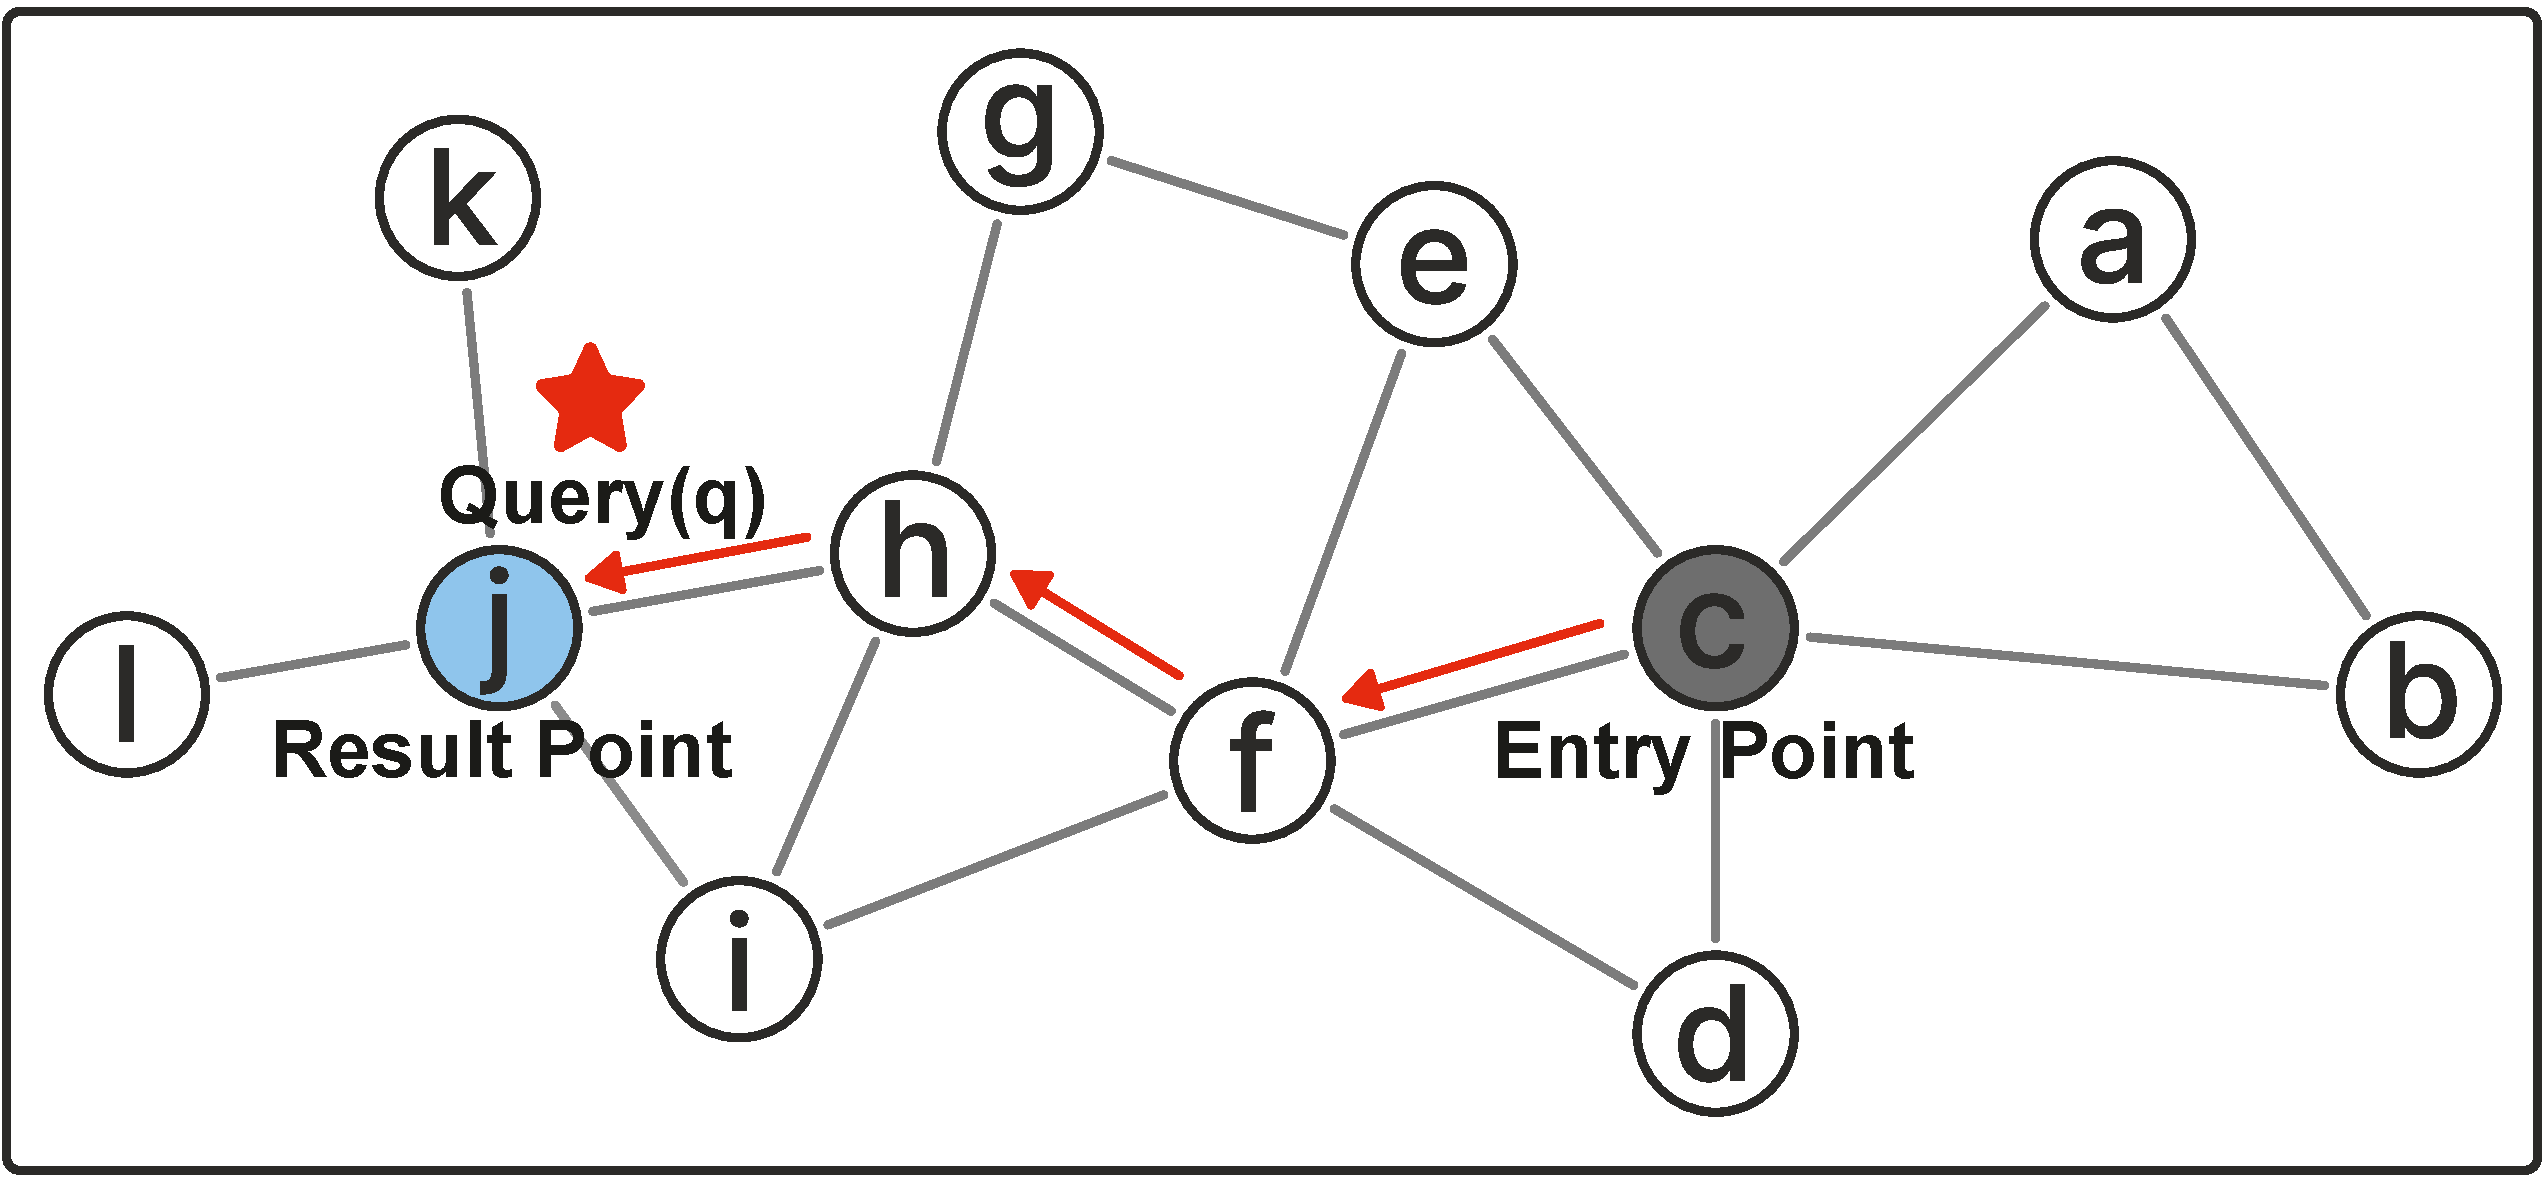
\includegraphics[width=\linewidth]{figures/graph.pdf}
			\caption{Graph Index}
			\label{fig:graph}
		\end{subfigure}
		\hfill
		\begin{subfigure}{0.38\columnwidth}
			\centering
			
			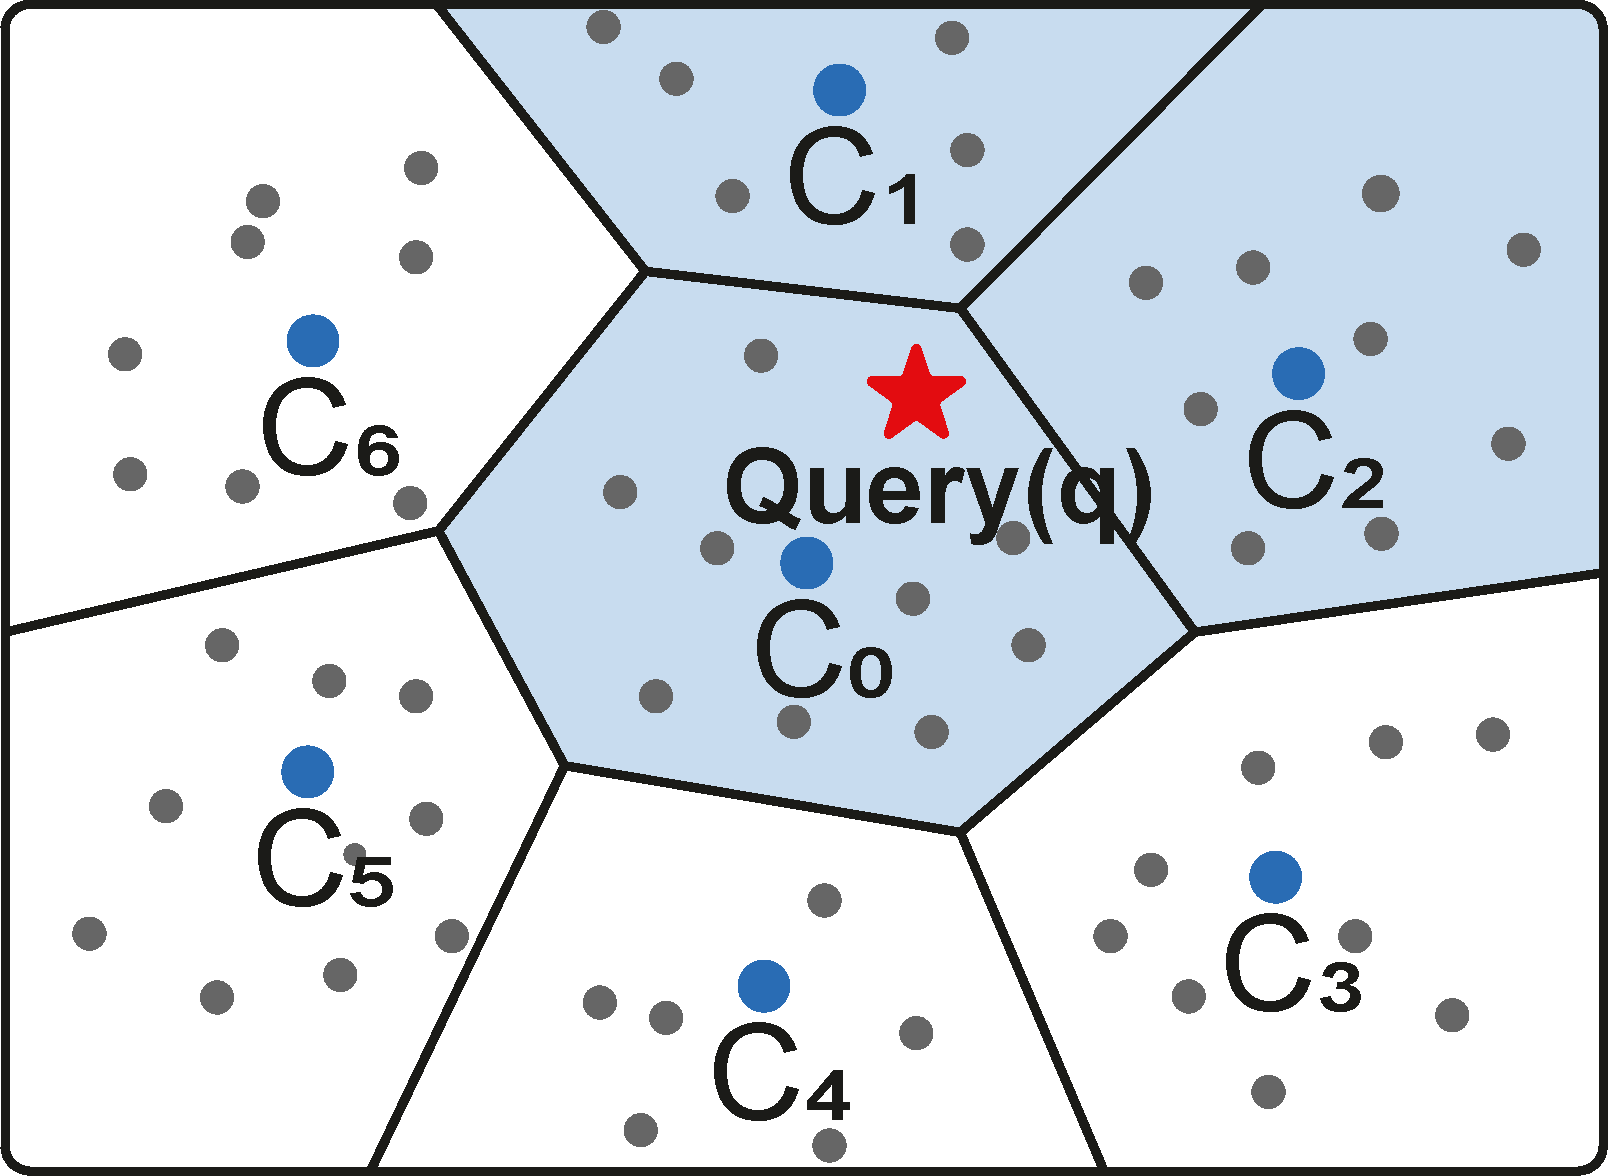
\includegraphics[width=\linewidth]{figures/ivf.pdf}
			\caption{IVF Index}
			\label{fig:ivf}
		\end{subfigure}
		
	\setlength{\abovecaptionskip}{0.15cm}
	\setlength{\belowcaptionskip}{-0.10cm}
		\caption{Graph Index and IVF Index}
		
	\end{figure}
	
	
	\section{Hybrid querying Algorithms}
	
	
	\renewcommand{\arraystretch}{0.9}
	\begin{table*}[t]
		\centering
		\setlength{\abovecaptionskip}{0.15cm}
		\setlength{\belowcaptionskip}{-0.1cm}
		%\setlength{\belowcaptionskip}{-0.3cm}
		
		\caption{\textcolor{black}{Overview of AF-ANN and RF-ANN Search Algorithms}}
		\small
	\label{tab:compair_1}
	\begin{tabular}{|l|l|*{12}{c|}}
		\hline
		
	
		\multicolumn{2}{|c|}{\textbf{Characteristics/Algorithms}} & \textbf{NHQ} & \textbf{Filtered} & \textbf{Stitched} & \textbf{CAPS} & \textbf{ACORN} & \textbf{UNG} & \textbf{Puck} & \textbf{DSG} & \textbf{iRange} & \textbf{SeRF} & \textbf{UNIFY} & \textbf{Win}
		 \\ \hline
%		\multirow{6}{*}{\centering\textbf{AF}} 
		\multirow{6}{*}{\raisebox{4ex}{\textbf{AF}}}
		%& Filter Type         & C   & C   & C   & C   & B   & B   & B   & \multicolumn{5}{c|}{} \\ \cline{2-9}
		& AND                 & Y   & N   & N   & Y   & Y   & Y   & Y   & \multicolumn{5}{c|}{\multirow{4}{*}{\centering\shortstack{AF\\Not Support}}} \\ \cline{2-9}
		& OR                  & N   & Y   & Y   & N   & Y   & Y   & Y   & \multicolumn{5}{c|}{} \\ \cline{2-9}
		& Flexible Attributes & N   & Y   & Y   & Y   & Y   & Y   & Y   & \multicolumn{5}{c|}{} \\ \cline{2-9}
		& Complex Boolean     & N   & N   & N   & N   & Y   & N   & N   & \multicolumn{5}{c|}{} \\ \hline
		
		\multicolumn{2}{|l|}{\textbf{RF}}             & N & N & N & N & Y & N & N & Y & Y & Y & Y & Y \\ \hline
			\multicolumn{2}{|l|}{\textbf{Filter Type }}             & C & C & C & C & B & B & B & B & B & B & A/B/C & A \\ \hline
		\multicolumn{2}{|l|}{\textbf{Dynamic Insert}} & N & Y & N & Y & Y & Y & Y & N & Y & Y & Y & Y \\ \hline
		\multicolumn{2}{|l|}{\textbf{Multi Thread}}   & N & Y & Y & Y & Y & Y & Y & N & Y & Y & Y & Y \\ \hline
		\multicolumn{2}{|l|}{\textbf{Disk Support}}           &N  & Y& N & N & N & N & N & N & N & N & N & N \\ \hline
		\multicolumn{2}{|l|}{\textbf{Base}}           & Graph & Graph & Graph & IVF & Graph & Graph & IVF & Graph & Graph & Graph & Graph & Graph \\ \hline
	\end{tabular}
		

		
		
		\centering
		\footnotesize{
			\begin{minipage}{\linewidth}


		\textcolor{black}{
		\textit{Filtered}: FilteredVamana, \textit{Stitched}: StitchedVamana, \textit{Win}: WinFilter.
		\textit{AND} / \textit{OR}: Whether the algorithm supports the corresponding logical operations.
		\textit{Flexible Attributes}: Allows the number of query attributes to differ from that in index construction.
		\textit{Complex Boolean}: Supports NOT or nested Boolean expressions.
		\textit{Dynamic Insert}: Supports dynamic data insertion.
		\textit{Multi Thread}: Supports multi-threaded search.
		\textit{Disk Support}: Supports disk-based storage.
		\textit{Base}: Underlying ANN index structure used.}
		\textit{A}: Post-filtering (Filter after ANN search), 
		\textit{B}: Pre-filtering (Filter before ANN search), 
		\textit{C}: Simultaneous filtering (Filter simultaneously with ANN search), 
		\textit{Y}: Support, 
		\textit{N}: Unsupport. 
		\end{minipage}}
		
	\end{table*}
	
	

	Table~\ref{tab:compair_1} provides a comparative overview of 6 attribute filtering and 5 representative range filtering algorithms. 
	
	\subsection{Attribute Filtering Algorithms}
	



	\noindent\textbf{\underline{NHQ} \footnote{https://github.com/KGLab-HDU/TKDE-under-review-Native-Hybrid-Queries-via-ANNS}}  \cite{NHQ}
	Traditional attribute filtering algorithms usually perform attribute constraints and ANN search separately. In contrast, NHQ is the first to implement simultaneous filtering, integrating both aspects into a unified framework. NHQ constructs an index based on a nearest neighbor graph and introduces a fusion distance that jointly captures vector similarity and attribute similarity. Leveraging this fusion distance, NHQ unifies vector similarity and attribute matching into a single comprehensive similarity measure and builds the graph accordingly. During the query process, NHQ efficiently prunes irrelevant edges via this composite index, enabling fast retrieval of results that satisfy both vector similarity and attribute constraints.
	
	\noindent\textbf{\underline{Filtered-DiskANN} \footnote{\textcolor{black}{https://github.com/microsoft/DiskANN}}} \cite{Filtered-diskann}
	Filtered-DiskANN also supports simultaneous filtering. Built upon the Vamana \cite{diskann} graph-based ANN index, it incorporates attribute information directly into the graph during index construction. This integration ensures that the index reflects both vector similarity and attribute constraints. 
	Filtered-DiskANN proposes two indexes:  
	1) \textbf{FilteredVamana}, which incrementally builds the graph index by inserting data points and dynamically adding edges, allowing adaptive expansion.  
	2) \textbf{StitchedVamana}, which adopts a batch construction strategy—constructing separate Vamana subgraphs for each attribute, followed by merging and edge pruning.

	
	
	\noindent\textbf{\underline{CAPS} \footnote{\textcolor{black}{https://github.com/gaurav16gupta/constrainedANN}}}\cite{CAPS}
	CAPS introduces a hierarchical sub-partitioning algorithm inspired by Huffman trees, termed the Attribute Frequency Tree (AFT), to overcome the coarse granularity of traditional IVF-based methods. It adopts a two-level partitioning strategy:  
	1) The first level clusters vectors based on similarity using K-Means or learning-based methods such as BLISS. 2) Within each cluster, AFT partitions data further based on attribute frequencies, enabling finer-grained indexing and improving query efficiency.
	
	\noindent\textbf{\underline{ACORN} \footnote{\textcolor{black}{https://github.com/stanford-futuredata/ACORN}}}
	\cite{ACORN}
	\textcolor{black}{ACORN adopts a predicate-agnostic indexing framework. It is based on Hierarchical Navigable Small World (HNSW) \cite{hnsw} and builds a denser hierarchical graph through neighborhood expansion and edge pruning.}
	During search, it filters out nodes violating constraints, maintaining a valid nearest neighbor graph.
	ACORN includes two indexes: 1) \textbf{ACORN-$\gamma$}, which expands neighbor lists during construction, trading memory for higher performance; 
	2) \textbf{ACORN-1}, which extends neighbor lists via second-hop neighbors during search, reducing index size with minor performance loss.
	
	\noindent\textbf{\underline{UNG} \footnote{\textcolor{black}{https://github.com/YZ-Cai/Unified-Navigating-Graph}}} \cite{UNG}
	UNG serves as a unified framework that integrates various graph-based ANN indexes to support hybrid queries. It first groups the dataset by attribute sets, ensuring that vectors in each group share identical attributes. Then, it constructs a Label Navigating Graph (LNG) to encode inclusion relationships among attribute sets. Within each group, UNG builds graph-based ANN indexes (e.g., Vamana, HNSW) and connects them via cross-group edges to enable efficient cross-group search.

	
	
	
	\noindent\textbf{\underline{Puck} \footnote{\textcolor{black}{https://github.com/baidu/puck}}} \cite{puck}
	Puck utilizes two-level quantization for indexing. It maintains an attribute set for each cluster to track vector attributes. During the query process, it employs pre-filtering to exclude clusters without required attributes, thereby reducing the search space.

	
	
	
	\subsection{Range Filtering Algorithms}
	
	\noindent\textbf{\underline{SeRF} \footnote{\textcolor{black}{https://github.com/rutgers-db/SeRF}}} \cite{serf} 
%	Conventional RF-ANN search approaches typically follow one of two paradigms: 1) Conducting ANN search first followed by attribute-based filtering. 2) Filtering the dataset based on attribute ranges before performing ANN search. 
	Building a separate neighbor graph (e.g., HNSW) for each attribute range could ensure efficient querying but incurs an $O(n^2)$ cost in constructing and storing $n$ graphs. Since many edges are shared across these graphs, SeRF introduces a validity-range aware design where each edge records the interval in which it is valid, indicating in which subgraphs the edge remains valid. This compresses $n$ graphs into a single unified graph, maintaining search effectiveness while significantly reducing memory and index construction overhead.
	
	\noindent\textbf{\underline{WinFilter} \footnote{\textcolor{black}{https://github.com/JoshEngels/RangeFilteredANN}}} \cite{winFilter}
%	Unlike SeRF, which focuses on graph compression, 
	WinFilter proposes a structural partitioning framework called the $\beta$-Window Search Tree ($\beta$-WST). After the dataset is sorted by attribute values, it is partitioned into multiple intervals and organized into a tree structure. Each node in the tree corresponds to an attribute range and maintains a local ANN index (e.g., Vamana). For a range filtering query, WinFilter only searches within nodes overlapping the query range and merges partial results. With a tree height of $O(\log n)$, each query accesses at most $O(\log n)$ sub-indexes, resulting in significant speedups.
	
	\noindent\textbf{\underline{iRange} \footnote{\textcolor{black}{https://github.com/YuexuanXu7/iRangeGraph}}} \cite{iRangeGraph}
%	To address the query efficiency degradation caused by the graph compression in SeRF, iRange adopts a more flexible strategy.
	%Rather than prebuilding indexes for all possible ranges, it dynamically assembles a query-specific subgraph at runtime.
	iRange partitions the dataset into intervals based on attribute values and independently constructs a local graph for each interval, storing only edge information. During the query process, the relevant local graphs overlapping with the query range are merged into a temporary search graph, and a pruning strategy is applied to enable efficient search.
	
	\noindent\textbf{\underline{DSG} \footnote{\textcolor{black}{https://github.com/rutgers-db/DynamicSegmentGraph}}}  \cite{DSG}
%	Most RF-ANN search methods, such as iRange and WinFilter, are designed for static datasets. SeRF allows incremental insertion but requires ordered attributes. 
	DSG introduces the first dynamic RF-ANN framework supporting data insertion with unordered attributes while maintaining efficient range filtering.
	DSG relies on two data structures: 1) A rectangle tree partitions query space into rectangular regions, each corresponding to a group of queries sharing nearest neighbors. 2) A dynamic segment graph is a neighbor graph where each edge is annotated with its valid attribute range.
	With these structures, only few regions need updates when inserting new data. The system considers only edges valid for current attribute range to boost efficiency during search.
	
	\noindent\textbf{\underline{UNIFY} \footnote{\textcolor{black}{https://github.com/sjtu-dbgroup/UNIFY}}} \cite{UNIFY}
%	Unlike DSG, which relies on rectangle trees and range-aware edges, UNIFY adopts a segmentation-based approach and proposes a range query index structure. 
	UNIFY introduces the Segmented Inclusive Graph (SIG), which partitions the dataset into segments by attribute and constructs an independent neighbor graph for each segment. These segment graphs are then integrated into a unified global graph. Its hierarchical variant, HSIG, enhances SIG by incorporating the multilayer design of HNSW, skip lists, and edge bitmaps for efficient range localization and post-filtering pruning. UNIFY supports 3 filtering strategies—pre-filtering, post-filtering, and  simultaneous filtering—enabling robust and flexible performance.
	
	
	
	\subsection{Vector Libraries and Databases}
The vector library and databases discussed in the following are not explicitly designed for hybrid query, but they support both attribute filtering and range filtering. 

\noindent\textbf{\underline{Faiss}\footnote{\url{https://github.com/facebookresearch/faiss}}}  \cite{Faiss}
Faiss is an efficient similarity search library. It supports hybrid search by using an ID selector to filter data before performing ANN search.
In Faiss, we use the HQI batch optimization strategy in the IVF index. It groups queries with the same filter conditions. Each group only runs the filter once. It uses efficient matrix operations to compute vector similarity in batches.

\noindent\textbf{\underline{PASE}\footnote{\url{https://github.com/alipay/PASE}}} \cite{pase}  PASE is a vector index plugin for PostgreSQL. It uses a post-filtering strategy. Since the candidate set size is fixed, it may fail to return enough top-k results.

\noindent\textbf{\underline{VBASE} \footnote{\url{https://github.com/microsoft/MSVBASE}}} \cite{vbase} VBASE is also a vector plugin for PostgreSQL. Unlike PASE, it applies filters during the HNSW index traversal, discarding unmatched nodes on the fly. This strategy ensures that enough valid results are returned .



\noindent\textbf{\underline{Milvus} \footnote{\url{https://github.com/milvus-io/milvus}}}  \cite{milvus} Milvus is a vector database designed for large-scale similarity search. In hybrid queries, it adopts a pre-filtering strategy, similar to the ID selector mechanism used in Faiss.
%It filters data first, then performs approximate nearest neighbor search. This supports hybrid search.

	
	\section{Experiments}
	\subsection{Experimental Setup}
	\subsubsection{Datasets}
	
	\textcolor{black}{Our experiments employ 12 real-world datasets: Audio~\cite{audio_unknown},  Enron~\cite{enron2015}, GIST1M~\cite{sift2010}, GloVe~\cite{GloVe2015}, Msong~\cite{msong2011}, SIFT1M\\~\cite{sift2010}, Deep1M~\cite{yandex_deep_dataset}, WIT-Real~\cite{wit_dataset}, YT-Audio-Real~\cite{youtube8m_dataset}, Text2image~\cite{texttoimage}, Text2image-Mix, and Deep100M.}
	
	Table~\ref{tab:datasets_combined} summarizes the key characteristics of all datasets and their applicable filtering scenarios. In particular, we report the Local Intrinsic Dimensionality (LID)~\cite{Lid}, which is a commonly used metric to quantify dataset hardness. Following the standard evaluation protocol~\cite{LID2}, we randomly sample 10,000 data points from each dataset to compute LID.  A higher LID value indicates a more complex dataset.
	
	\textcolor{black}{The first 7 datasets are widely used in existing studies, while the remaining are common datasets with added real attributes. As they do not inherently come with attributes, we generate attributes for them to precisely control attribute quantity and distribution. WIT-Real and YT-Audio-Real datasets use real attributes. For the WIT-Real dataset, we use the CLIP model to encode the page title into vectors, and extract the language type and the length of the context page description  as real attributes. The YT-Audio-Real dataset uses YouTube8M data, employing the video category ID and view counts as real attributes.}
	
	\textcolor{black}{Additionally, we use the Out-of-Distribution (OOD) dataset Text2-Image and the large-scale dataset Deep100M to evaluate the generalization capability of the algorithms. The Text2Image dataset includes two versions. The original version contains 1 million image embeddings as the base dataset and uses 10 thousand text embeddings as the query set. The Text2Image-Mix version is composed of 0.5 million image embeddings and 0.5 million text embeddings as the base dataset, with a query set of 5 thousand image embeddings and 5 thousand text embeddings.}
	

	

	
	
	\renewcommand{\arraystretch}{0.9}
	\begin{table}[t]
		\centering
		\setlength{\abovecaptionskip}{0.15cm}
		\setlength{\belowcaptionskip}{-0.1cm}
		
		
		\caption{Datasets}
		
		\label{tab:datasets_combined}
		\resizebox{\columnwidth}{!}{
			\begin{tabular}{ccccccc}
				\toprule
				Dataset & Dimension & Base Data & Queries & LID & Type& Used \\
				\midrule
				
				Audio & 192 & 53,387 & 200 & 14& Audio& AF \\
				Enron & 1369 & 94,987 & 200 & 23& Text& AF \\
				GIST1M & 960 & 1,000,000 & 1,000 & 45& Image& AF \\
				GloVe & 100 & 1,183,514 & 10,000 & 47& Text& AF \\
				Msong & 420 & 992,272 & 200 & 23& Audio& AF \\
				SIFT1M & 128 & 1,000,000 & 10,000 & 19& Image& AF \\
				
				%YT-Audio& 128 & 1,000,000 & 10,000 & 15& Audio \\
				Deep1M & 96 & 1,000,000 & 10,000 & 22 & Image& RF \\
				WIT-Real & 512 & 1,000,000 & 40,300 & 48& Image& Both \\
				YT-Audio-Real& 128 & 1,000,000 & 10,000 & 15& Audio& Both \\
				Text2Image & 200 & 10,000,000 &10,000 & 59& Text,Image& Both \\
				Text2Image-Mix & 200 & 1,000,000 &10,000 & 21& Text,Image& Both \\
				Deep100M & 96 & 100,000,000 & 10,000 & 22& Image& Both \\
				\bottomrule
			\end{tabular}
		}
	\end{table}
	
	
	
	
	
	
	\subsubsection{Evaluation Metrics}
	
	To assess the overall performance of different algorithms, we adopt a multi-dimensional quantitative evaluation framework~\cite{compare}, including the following 5 core metrics:
	
	\begin{enumerate}
		
		\item \textbf{Recall@k}: The proportion of overlap between the returned approximate $k$ nearest neighbors and the ground truth $k$ nearest neighbors.
		\item \textbf{QPS (Queries Per Second)}: The number of queries processed per second.
		\item \textbf{Index Construction Time}: The total time required to transform the raw dataset into a queryable index structure.
		\item \textbf{Index Size}: The storage size of the persisted index on disk.
		\item \textbf{Peak Memory Usage}: The maximum memory consumption observed during index construction \textcolor{black}{and search}.
	\end{enumerate}
	

	
	
	
	\subsubsection{\textcolor{black}{Setting}}
	
	
	We conduct most experiments on a server running Ubuntu 20.04, equipped with an AMD EPYC 7K62 processor (2.6GHz) featuring 256GB of RAM and 192 MiB of L3 cache. \textcolor{black}{We test on  large-scale dataset using a server with 2×AMD 7Y43 processors and 1TB RAM.}
%	\textcolor{cyan}{Additionally, to investigate the impact of different server configurations on algorithm performance, we also conducted partial experiments on a server equipped with dual Intel(R) Xeon(R) Gold 6330 CPU @ 2.00GHz and 128GB of RAM. For clarity and conciseness, we hereafter refer to the former as Server A and the latter as Server B. Unless otherwise specified, all experiments were conducted on Server A.} 
	Unless otherwise stated, we execute index construction with 32 threads to accelerate the process. The queries are all executed on a single thread. 
%	In addition, We summarize the multi-threading capabilities of each algorithm in Table~\ref{tab:compair_1}. 	For vector database systems, we adopt a multi-process evaluation scheme (rather than multi-threaded execution), following the methodology proposed in VectorDBBench~\cite{VectorDBBench}, to better reflect their real-world performance.
	
	\textcolor{black}{
	Regarding experimental parameter selection, we adopt the recommended settings from original papers when available. For datasets without suggested parameters, we test different configurations and select relatively optimal ones for final evaluation. Due to the large number of datasets and algorithms involved, specific parameters are not individually listed in the paper but are fully provided in our code repository.
}
%	\textcolor{black}{
%	\subsubsection{Parameters}
%	In the experiments, for datasets with recommended parameters in the original paper, we use the recommended settings. For datasets without recommended parameters, we conduct experiments with different parameter settings and select the one that performs best for the final experiment. Due to the large number of datasets and algorithms involved, the parameters are not listed individually, but they are provided in the code repository.
%}
	
	
	%4.2
	\subsection{Attribute Filtering}
	
	
	%4.2.1
	\subsubsection{\textcolor{black}{Time and Space overhead}}
	% \subsubsection{\textbf{Attribute Filtering}}
	\begin{figure}[t]
		\centering
		
		
		
		% 上面的图例,居中并可通过 hspace 调整左右位置
		\hspace*{8pt} % 可调整的参数,负值左移,正值右移,例如 -20pt 或 20pt
		
\includegraphics[width=0.95\columnwidth]{figures/indexData/legend_only.png} % 图例图片路径
		
		
		\begin{subfigure}{\columnwidth}
			\centering
			
			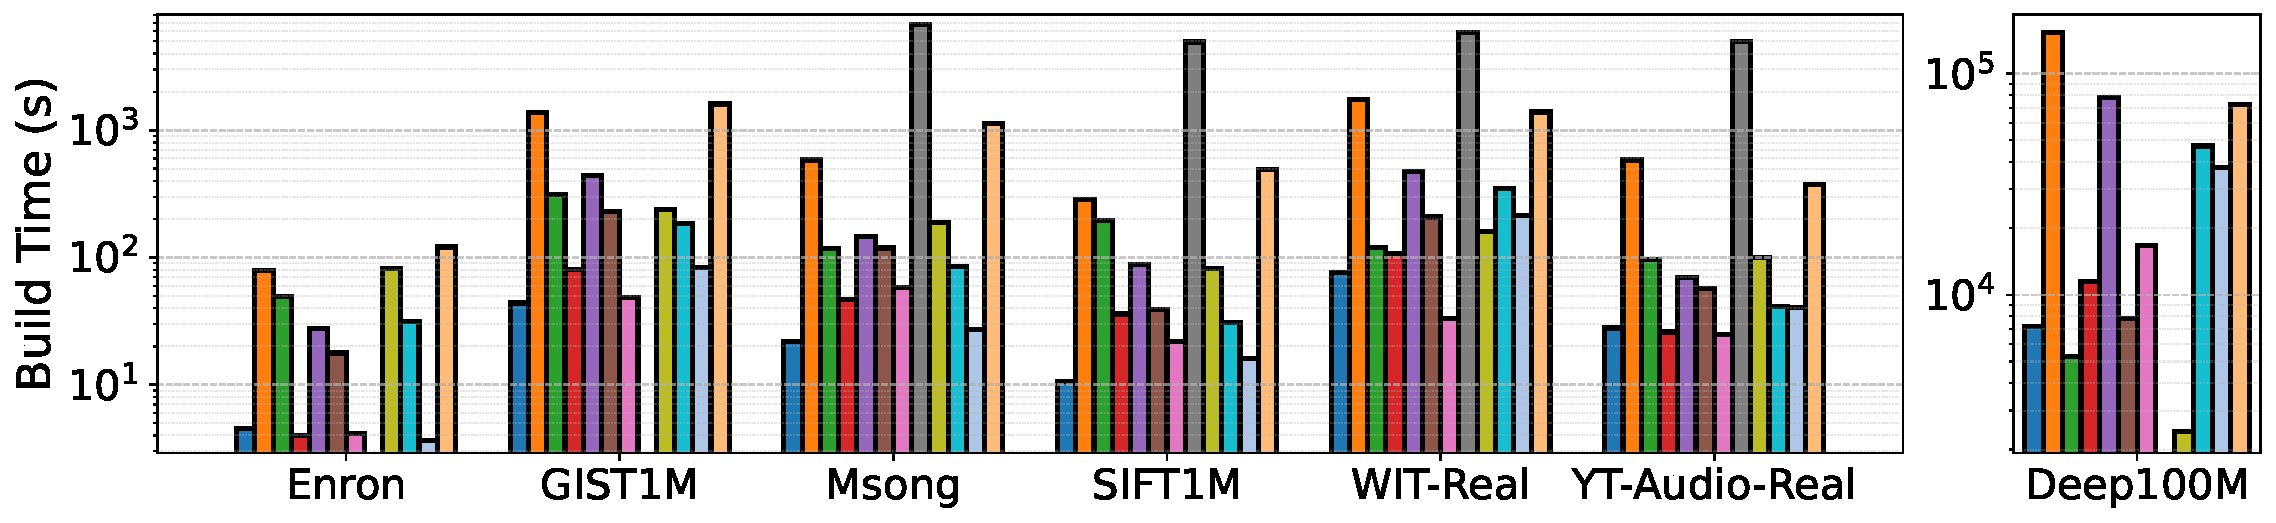
\includegraphics[width=0.99\linewidth]{figures/indexData/exp_7_build_time_comparison_query1.pdf}
			\caption{Construction Time}
			\label{fig:build_time_comparison_query1}
		\end{subfigure}
		
		
		
		\begin{subfigure}{\columnwidth}
			\centering
			
			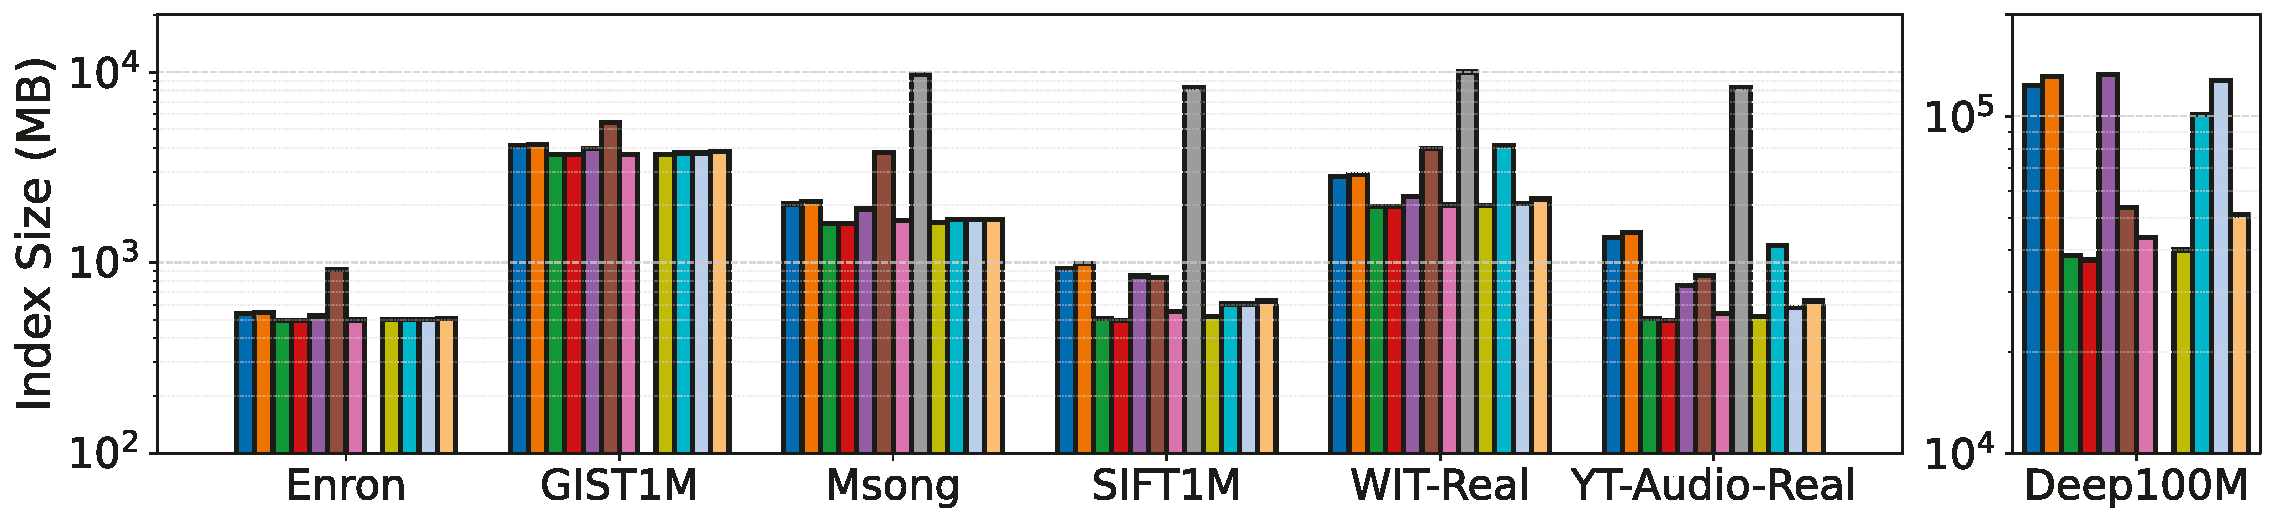
\includegraphics[width=0.99\linewidth]{figures/indexData/exp_7_index_size_mb_comparison_query1.pdf}
			\caption{Index Size (Including Original Dataset)}
			\label{fig:index_size_mb_comparison_query1}
		\end{subfigure}
		
		
		
		\begin{subfigure}{\columnwidth}
			\centering
			
			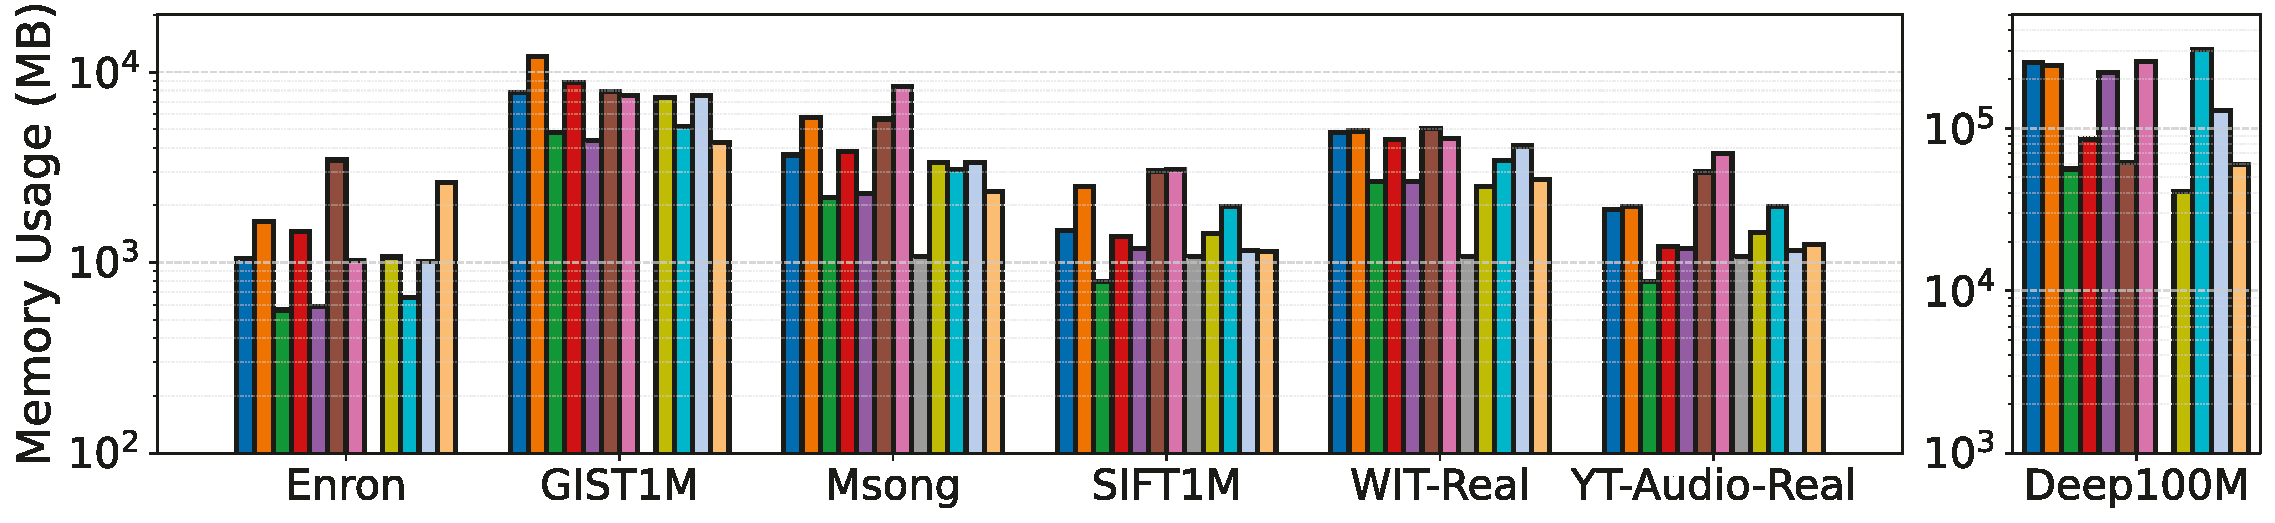
\includegraphics[width=0.99\linewidth]{figures/indexData/exp_7_memory_mb_comparison_query1.pdf}
			\caption{Build Peak Memory }
			\label{fig:build_memory_mb_comparison}
		\end{subfigure}
		
		\begin{subfigure}{\columnwidth}
			\centering

			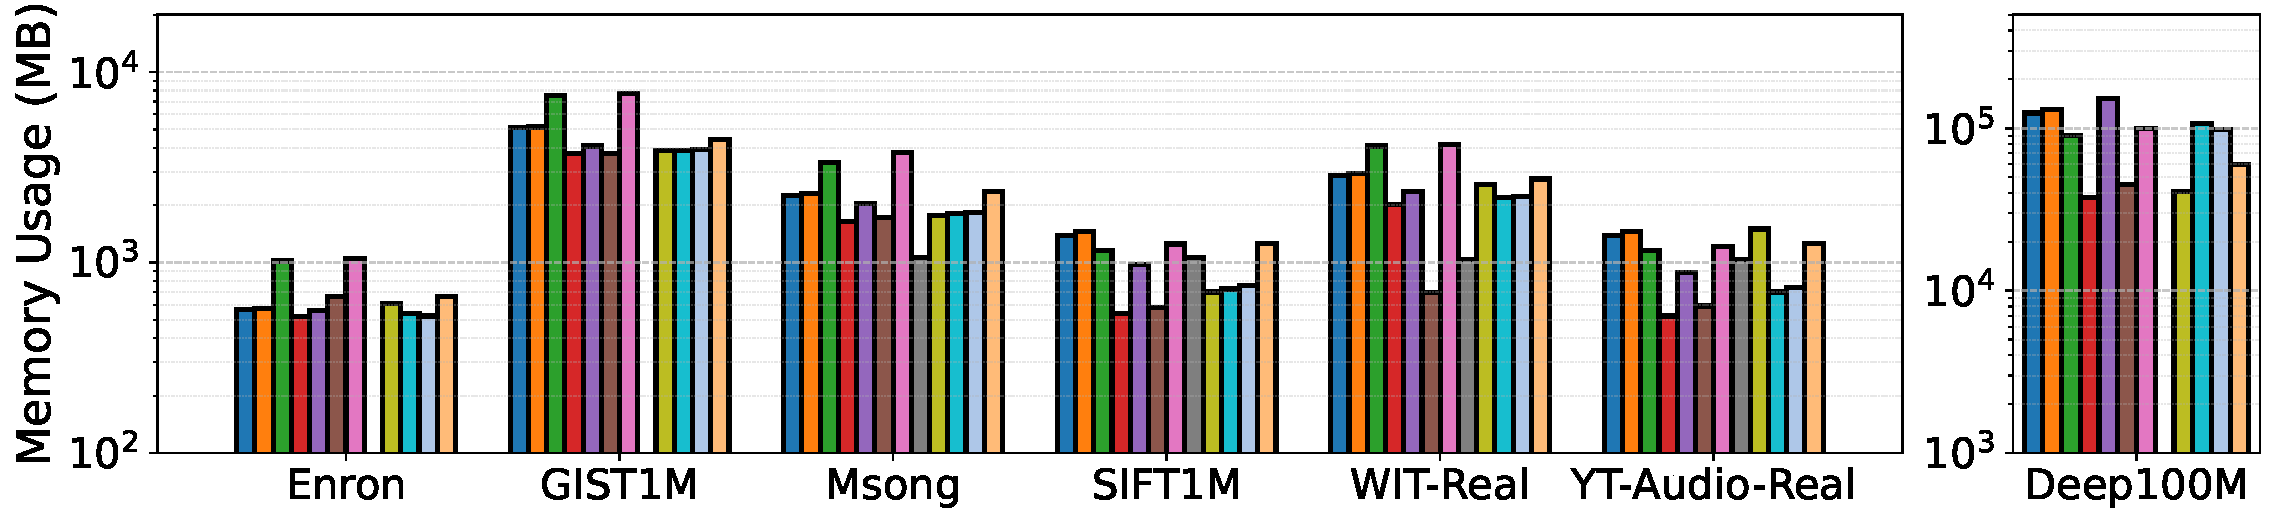
\includegraphics[width=0.99\linewidth]{figures/searchMem/label_memory_comparison.pdf}
			\caption{Search Peak Memory}
			\label{fig:search_memory_mb_comparison}
		\end{subfigure}
		
		%		\caption{Time and space overhead of attribute filtering index construction}
		\setlength{\abovecaptionskip}{0.15cm}
		\setlength{\belowcaptionskip}{-0.10cm}
		\caption{\textcolor{black}{Time and Space Overhead (AF)}}
		\label{fig:build_index_comparison}
	\end{figure}
	
	
	
	\textcolor{black}{To investigate the time and space overhead of different algorithms,} we evaluate \textcolor{black}{4} key metrics in the single-attribute scenario: index construction time, index size, \textcolor{black}{build peak memory and search peak memory}. Notably, PASE on GIST1M and Enron is omitted, as it supports only data with dimensionality less than 512. Furthermore, we did not measure PASE on large-scale datasets, as we estimated it would take over 10 days. \textcolor{black}{We use 64 threads to build the index for the large-scale Deep100M dataset, and 32 threads for the other 6 medium-scale datasets. Notably, the VBASE and PASE algorithms only support single-threaded construction.}
	
	
	\begin{figure*}
		\centering
		\setlength{\abovecaptionskip}{0.15cm}
		\setlength{\belowcaptionskip}{-0.10cm}
		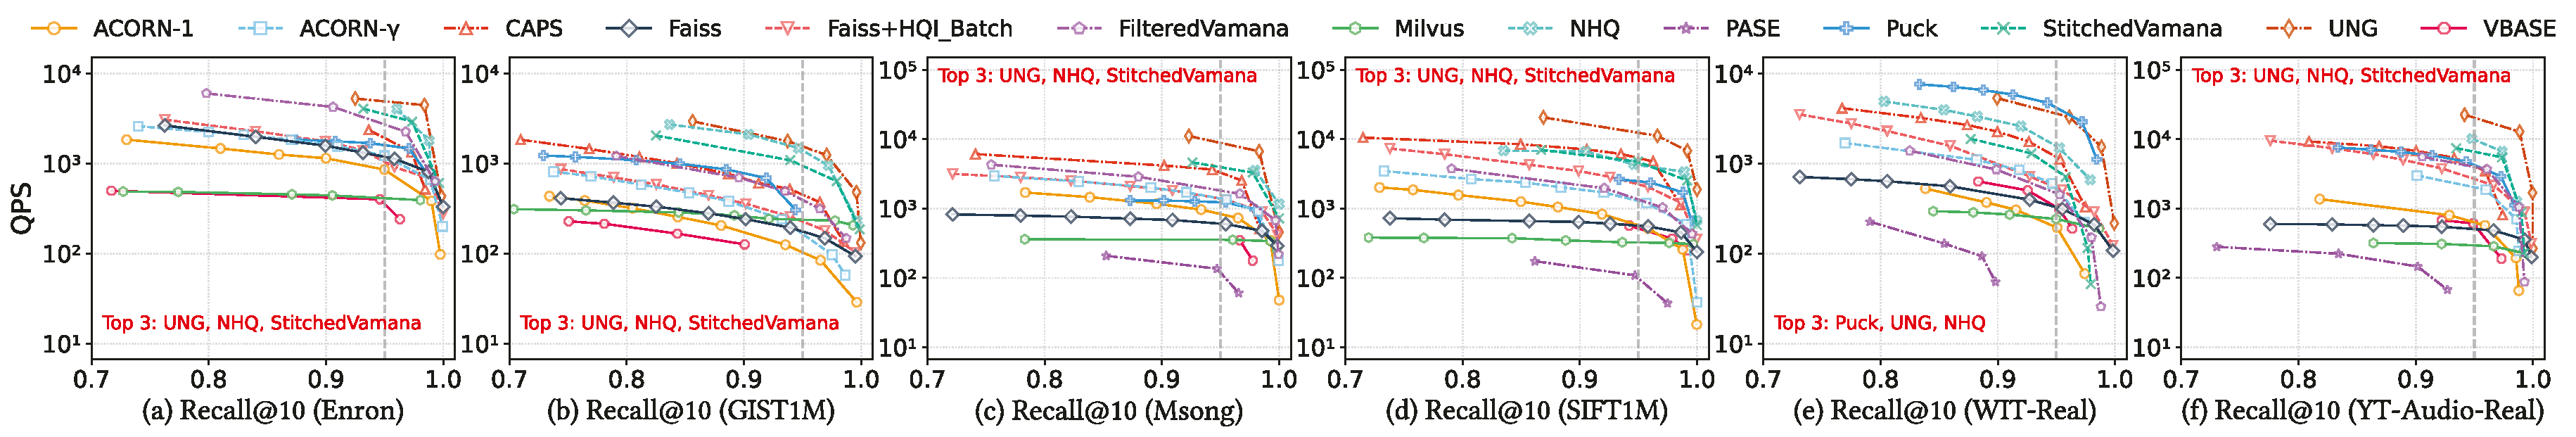
\includegraphics[width=0.95\textwidth]{figures/exp/exp_1_1_SingleLabel_1thread.pdf}
		\caption{Performance of Single-Attribute Index Construction and Single-Attribute Query }
		\label{fig:exp_1_1_SingleLabel_1thread}
	\end{figure*}
	
%	\begin{figure*}
%		\centering
%		
%		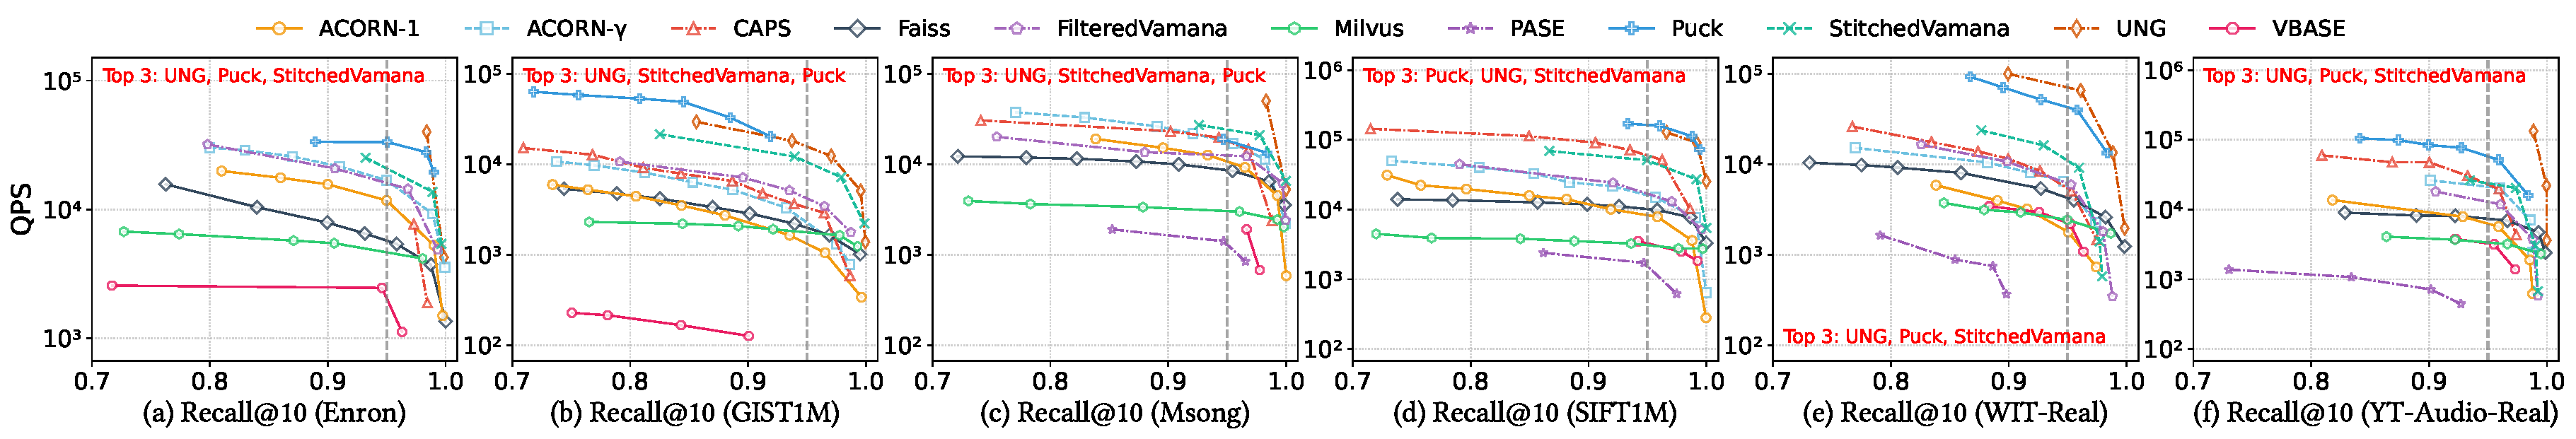
\includegraphics[width=0.95\textwidth]{figures/exp/exp_1_2_SingleLabel_16thread.pdf}
%%		\caption{Single-Attribute Building and Query performance (16 threads)}
%		\caption{Performance of Single-Attribute Index Construction and Single-Attribute Query (16 Threads)}
%		\label{fig:exp_1_2_SingleLabel_16thread}
%	\end{figure*}
	
\textit{\textbf{Index construction time.}}
\textcolor{black}{On the medium-scale datasets (Figure~\ref{fig:build_time_comparison_query1} left), among the algorithms limited to single-threaded construction, PASE has the longest build time. This is because its on-demand loading and caching strategies frequently trigger disk I/O and page scheduling, which seriously affects efficiency. In contrast, VBASE uses full-memory builds and is therefore comparatively faster. Among the multi-threaded algorithms, ACORN-$\gamma$ is the slowest because it needs to expand the neighbor list and evaluate a large number of candidates. Its build time on some datasets even exceeds that of the single-threaded VBASE. }

\textcolor{black}{On the large-scale dataset Deep100M (Figure~\ref{fig:build_time_comparison_query1} right), in addition to the three methods already mentioned, we also observe that algorithms based on Vamana (FilteredDiskANN, StitchedVamana and UNG) exhibit significantly increased construction time. This is because Vamana adopts a two-pass graph construction and optimization strategy (greedy search + robust pruning), resulting in extremely high computational overhead. In contrast, the construction time of IVF-based algorithms grows much more slowly with dataset size. This is because their shard-based design and high parallel efficiency, making them more scalable and advantageous in large-scale scenarios.}



\textit{\textbf{Index size.}}
\textcolor{black}{
	As shown in Figure~\ref{fig:index_size_mb_comparison_query1}, PASE exhibits significantly larger index sizes across all supported datasets, mainly due to its reliance on a large amount of metadata. For medium-scale datasets, other methods show moderate variation. However, on large-scale dataset, Graph-based algorithms such as ACORN, FilteredDiskANN, and UNG tend to exhibit a sharp increase in index size, primarily due to the large number of candidate neighbors they maintain. Overall, IVF-based methods tend to produce more compact indexes.
}


\textcolor{black}{\textit{\textbf{Peak memory.}}	
We present the peak memory usage during index construction and query processing in Figure~\ref{fig:build_memory_mb_comparison} and Figure~\ref{fig:search_memory_mb_comparison}, respectively. We observe that peak memory usage is generally correlated with the combined size of the index and the dataset. Methods that produce larger indexes tend to consume more memory during both construction and querying, and this trend holds consistently across different datasets.}

\textcolor{black}{However, there are notable exceptions. During index construction, PASE adopts an on-demand loading strategy, resulting in build peak memory usage even lower than the final index size. NHQ generates a large number of candidate neighbors during construction but retains only a small subset per node in the final index, leading to high peak memory usage despite a relatively compact index.
During querying, CAPS maintains a large candidate set dynamically, which significantly increases its search peak memory consumption.}


 
	\subsubsection{Performance Evaluation}
	
	
	%4.2.2
	
	
	We next evaluate the query performance of AF-ANN search methods, focusing on 3 main scenarios.
	
	\textit{\textbf{Single-Attribute Index Construction and Single-Attribute Query.}}
	In this scenario, we construct the index using an attribute and apply filtering conditions on the same attribute.
	
	
	
	As shown in Figure~\ref{fig:exp_1_1_SingleLabel_1thread}, as recall approaches 1, search often requires traversing larger candidate sets or deeper graph paths. This leads to increased computational cost and a sharp QPS drop for most methods. Despite this, UNG consistently maintains high QPS due to its LNG structure, which eliminates unnecessary online filtering of irrelevant attributes and searches only within the subgraph formed by points satisfying the filtering conditions, thereby improving query efficiency.
	
	\textcolor{black}{NHQ and StitchedVamana also perform well and show similar and stable performance across all datasets. This indicates that joint filtering and search strategies can achieve consistent effectiveness under high-recall requirements.} StitchedVamana outperforms FilteredVamana in query efficiency. This difference stems from their pruning strategies: StitchedVamana applies pruning after merging graphs, allowing nodes to accumulate a richer candidate set; while FilteredVamana applies early pruning, potentially eliminating useful candidates prematurely.
	%	Puck and CAPS perform relatively well. Partition-based methods have limitations regarding different vector data distributions, and how to configure different partitions for different datasets remains a challenge. However, this also demonstrates that IVF-based methods remain very promising for hybrid queries.
	\textcolor{black}{Additionally, Puck and CAPS also perform relatively well. They further reduce the search space on IVF indexes by using attribute partitioning, thereby achieving solid search performance.}
	
	Among all methods, vector database systems (PASE, VBASE, Milvus) show the worst performance. These systems target general-purpose scenarios but incur communication latency from network I/O and experience high query processing overhead due to complex query parsing. Additionally, we observe that Faiss+HQI\_Batch outperforms original Faiss, indicating that batch querying via HQI can effectively enhance query performance.
	

	
	\textit{\textbf{Multi-Attribute Index Construction and Single-Attribute Query.}}
	In this scenario, the index is constructed using 8 attributes but applies filtering condition on only 1 attribute during the query.
	
	Faiss offers an ID filtering mechanism, it operates solely during query execution and does not influence index building. ACORN is   designed for single-attribute indexing. In database systems (VBASE, PASE, Milvus), 
	%\sout{when the system builds both B+ tree and vector indexes, queries typically utilize only the B+ tree.} 
	attributes do not participate in index construction.
	Hence, they are excluded from this comparison.
	
	\begin{figure}[t]
		\centering
		\setlength{\abovecaptionskip}{0.15cm}
		\setlength{\belowcaptionskip}{-0.10cm}
		% 上面的图例,居中并可通过 hspace 调整左右位置
		\hspace*{15pt} % 可调整的参数,负值左移,正值右移,例如 -20pt 或 20pt
		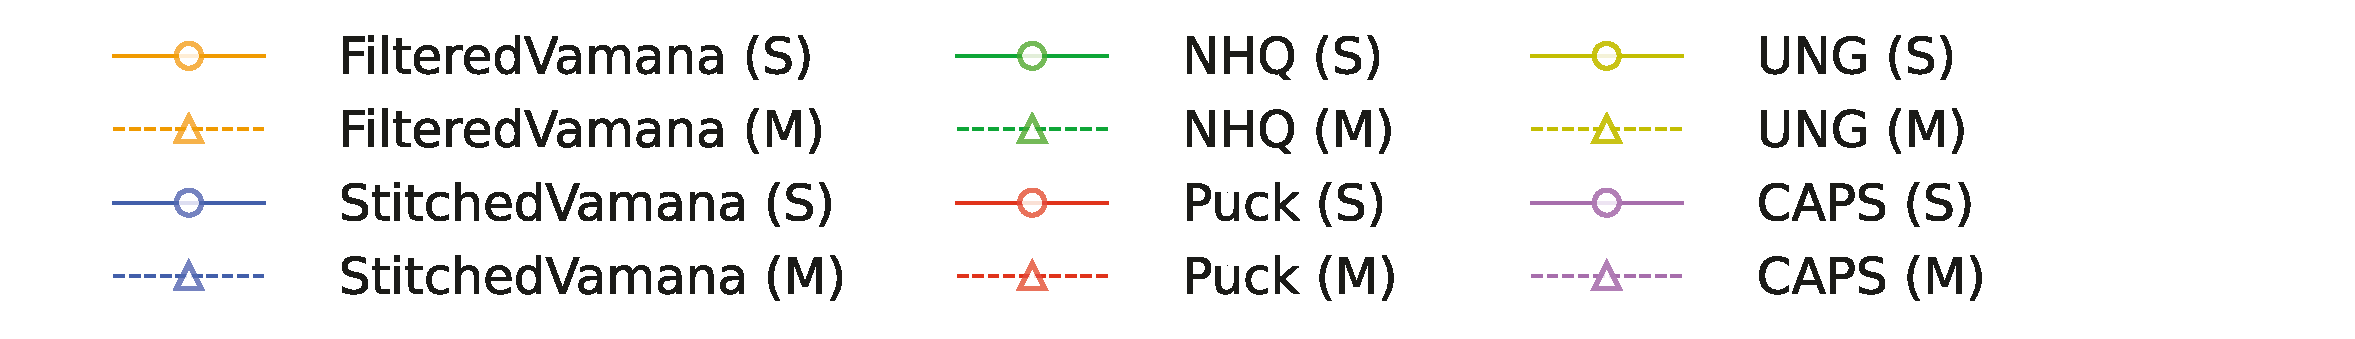
\includegraphics[width=0.85\columnwidth]{figures/exp/exp_2_legend.pdf} % 图例图片路径
		
		
		% 下面的子图,居中显示
		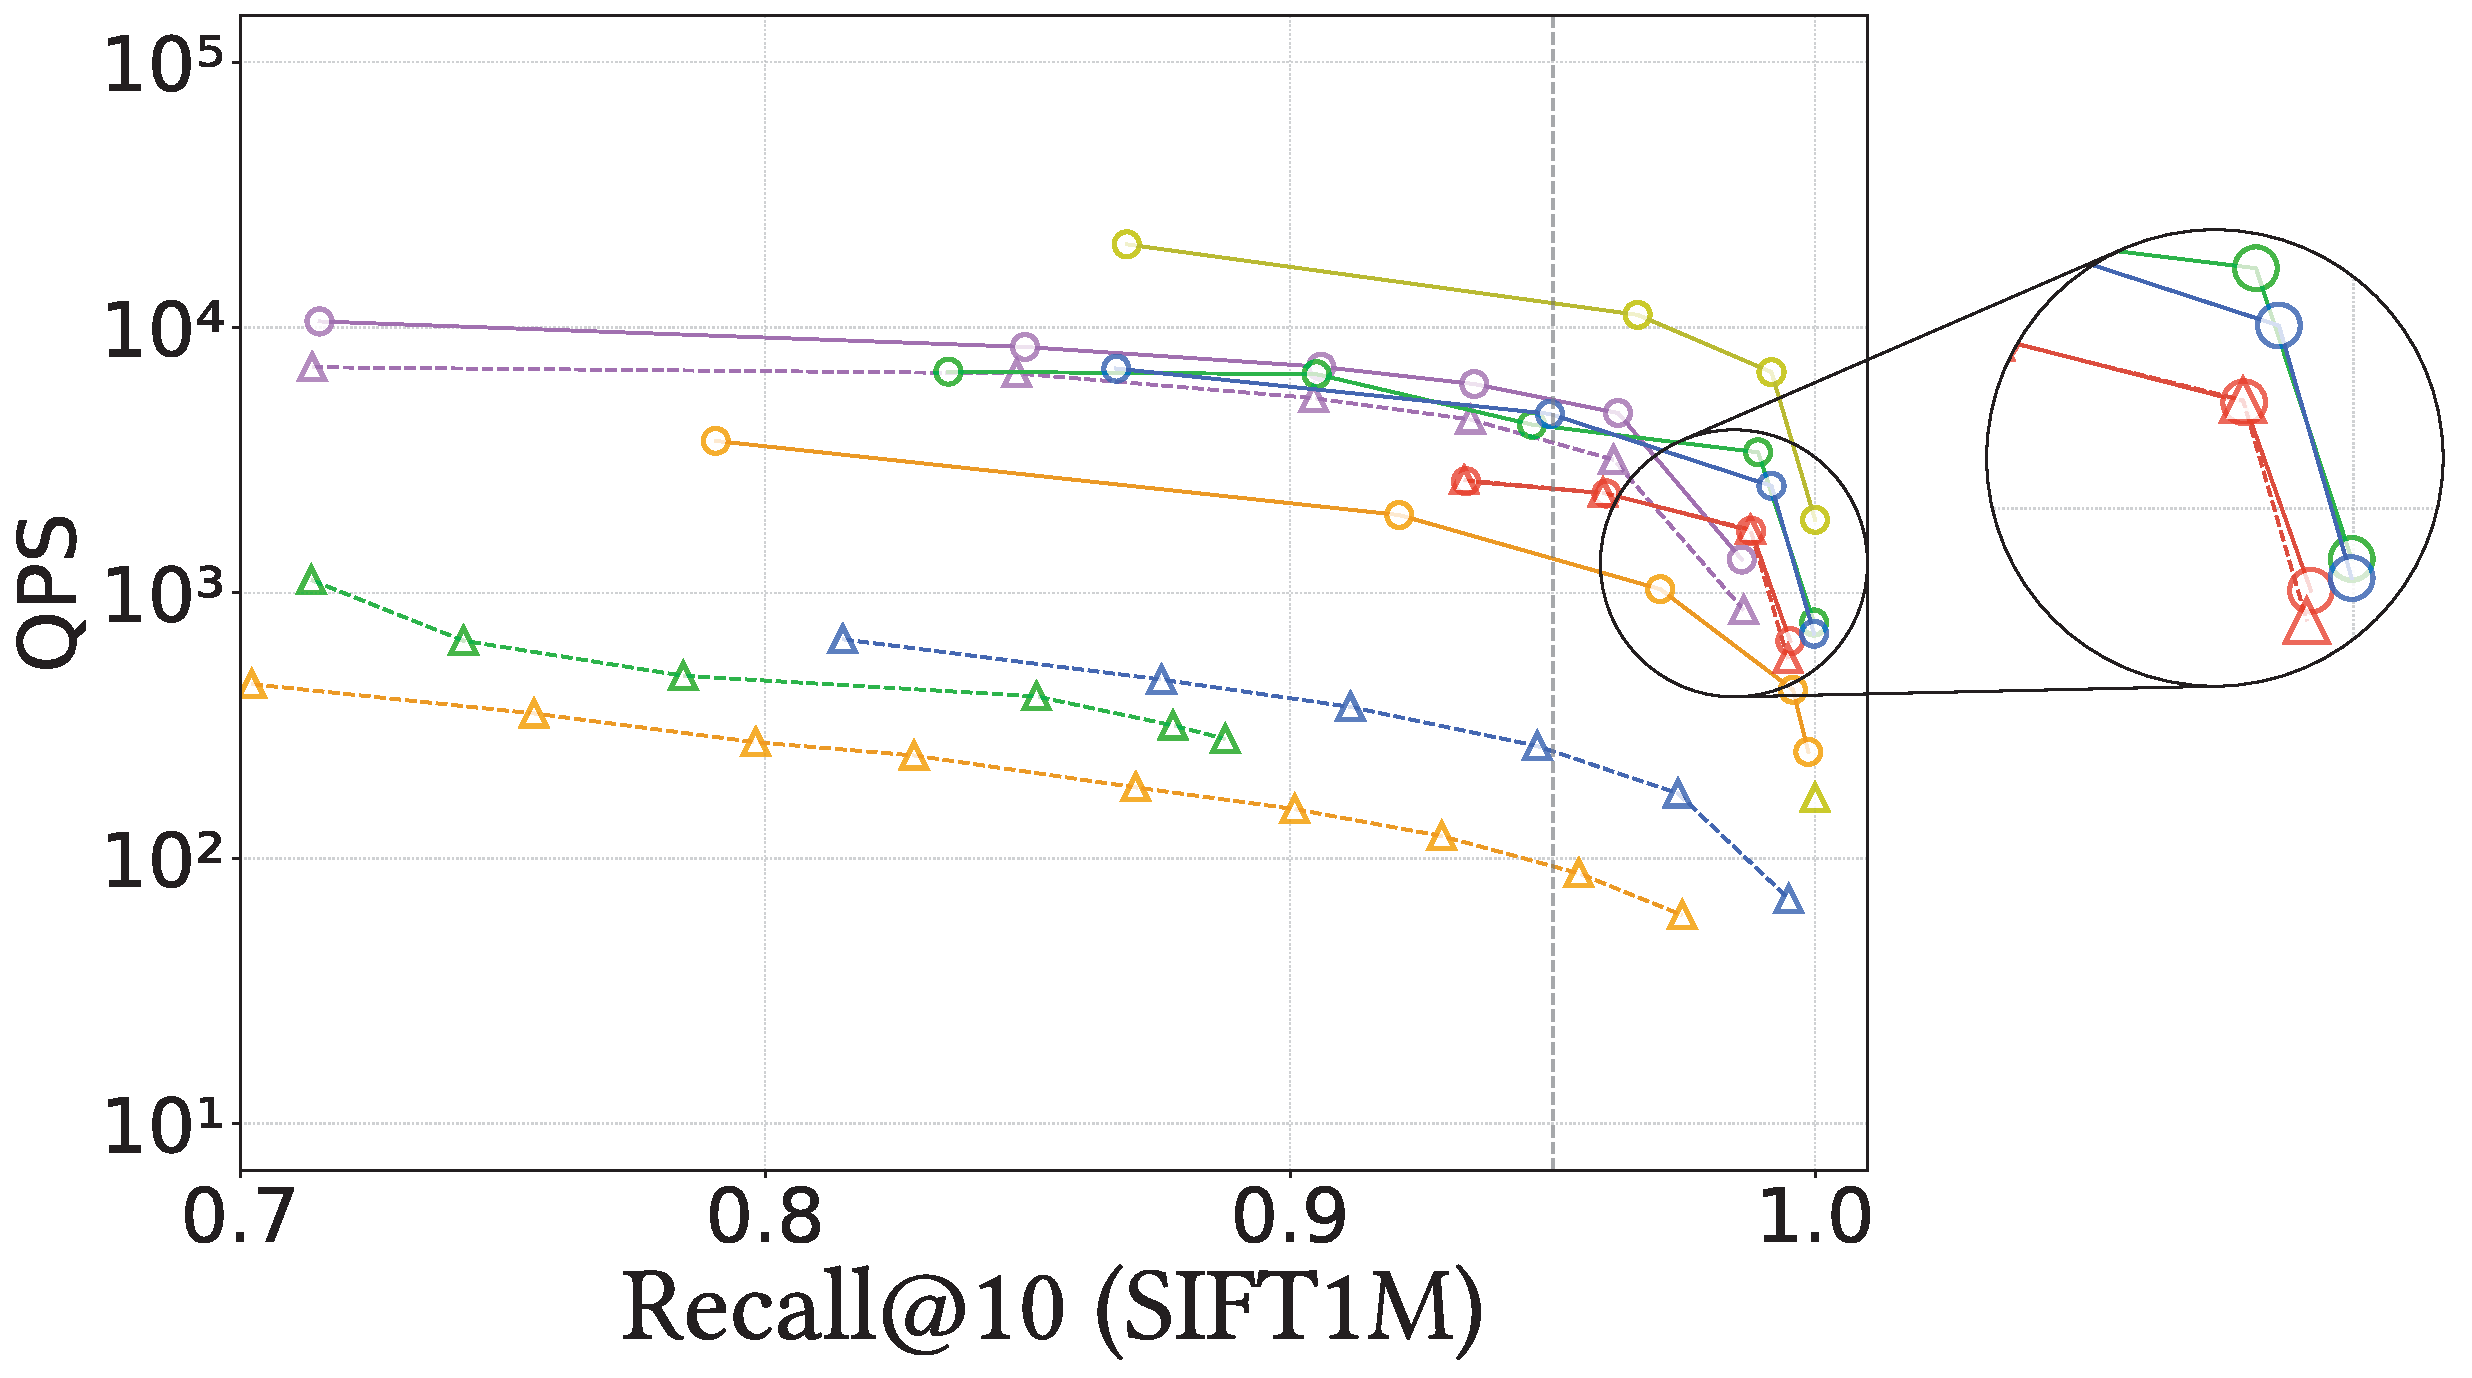
\includegraphics[width=0.7\columnwidth]{figures/exp/exp_2_1.pdf}
		\caption{Effect of Multi-Attribute Index Construction on Single-Attribute Query Performance ($S$ denotes single-attribute index construction and single-attribute query, $M$ denotes multi-attribute index construction and single-attribute query)}
		\label{fig:exp_2_1}
		
	\end{figure}
	
	(1) \textit{Effect of Multi-Attribute Building on Algorithm Performance (M vs. S).}
	As shown in Figure \ref{fig:exp_2_1}, Puck demonstrates nearly no performance degradation. CAPS shows a slight performance decline due to the increased query overhead caused by excessive attribute-based grouping. In contrast, the performance of StitchedVamana, FilteredVamana, NHQ, and UNG drops significantly, with the following reasons: 1) FilteredVamana increases the complexity introduced by retaining attribute during index construction. 2) The complexity of StitchedVamana increases because data points may duplicate across multiple subgraphs. 3) The fusion distance of NHQ exhibits sensitivity to the number of attributes, which degrades its effectiveness. 4) UNG has poor performance because large number of entry points that need to be traversed. It is difficult for a graph with multiple entries to have good connectivity, degenerating into a situation closer to inverted retrieval, and the effect may be greatly impaired.
	
	
	
	(2) \textit{Performance of Algorithms under Multi-Attribute Building (M vs. M).}  
	As shown in Figure \ref{fig:exp_2_1}, IVF-based methods (Puck and CAPS) significantly outperform graph-based methods. The reason for their superior performance is that they filter out irrelevant results during the retrieval process rather than searching for more candidates. In contrast, multi-attribute construction significantly degrades the performance of graph-based methods, for which we identify the primary reason. 
	\textcolor{black}{For algorithms with tightly coupled attribute and graph structures, increasing the number of attributes during index construction increases graph complexity. This makes single-attribute queries more difficult and degrades performance.}

	
	
	\begin{figure*}
		\centering
		\setlength{\abovecaptionskip}{0.15cm}
		\setlength{\belowcaptionskip}{-0.10cm}
		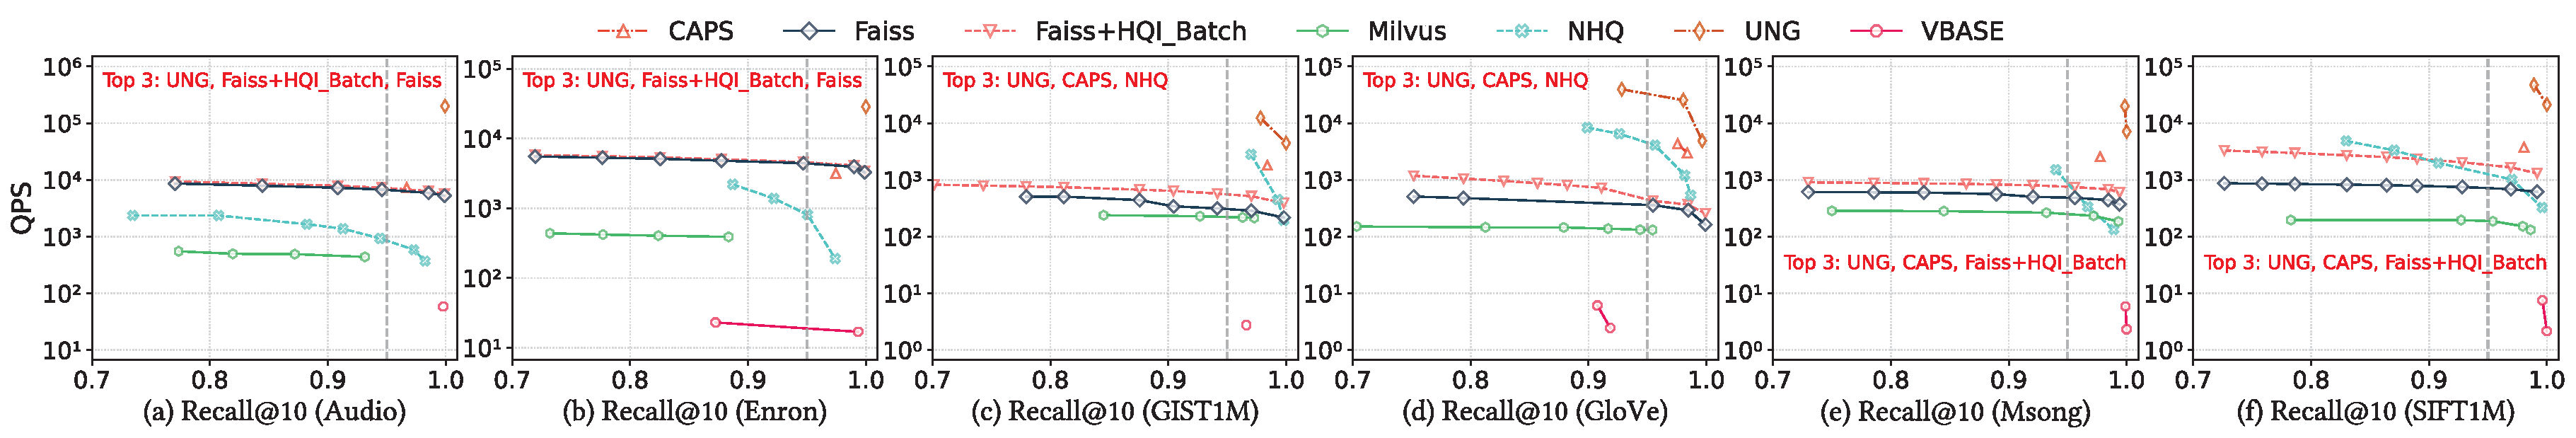
\includegraphics[width=0.95\textwidth]{figures/exp/exp_4_1_MultiLabel_1thread.pdf}
		\caption{Performance of Multi-Attribute Index Construction and Multi-Attribute Query}
		\label{fig:exp_4_1_MultiLabel_1thread}
	\end{figure*}
	
	
	\begin{figure*}
	\centering
	\setlength{\abovecaptionskip}{0.1cm}
	\setlength{\belowcaptionskip}{-0.25cm}
	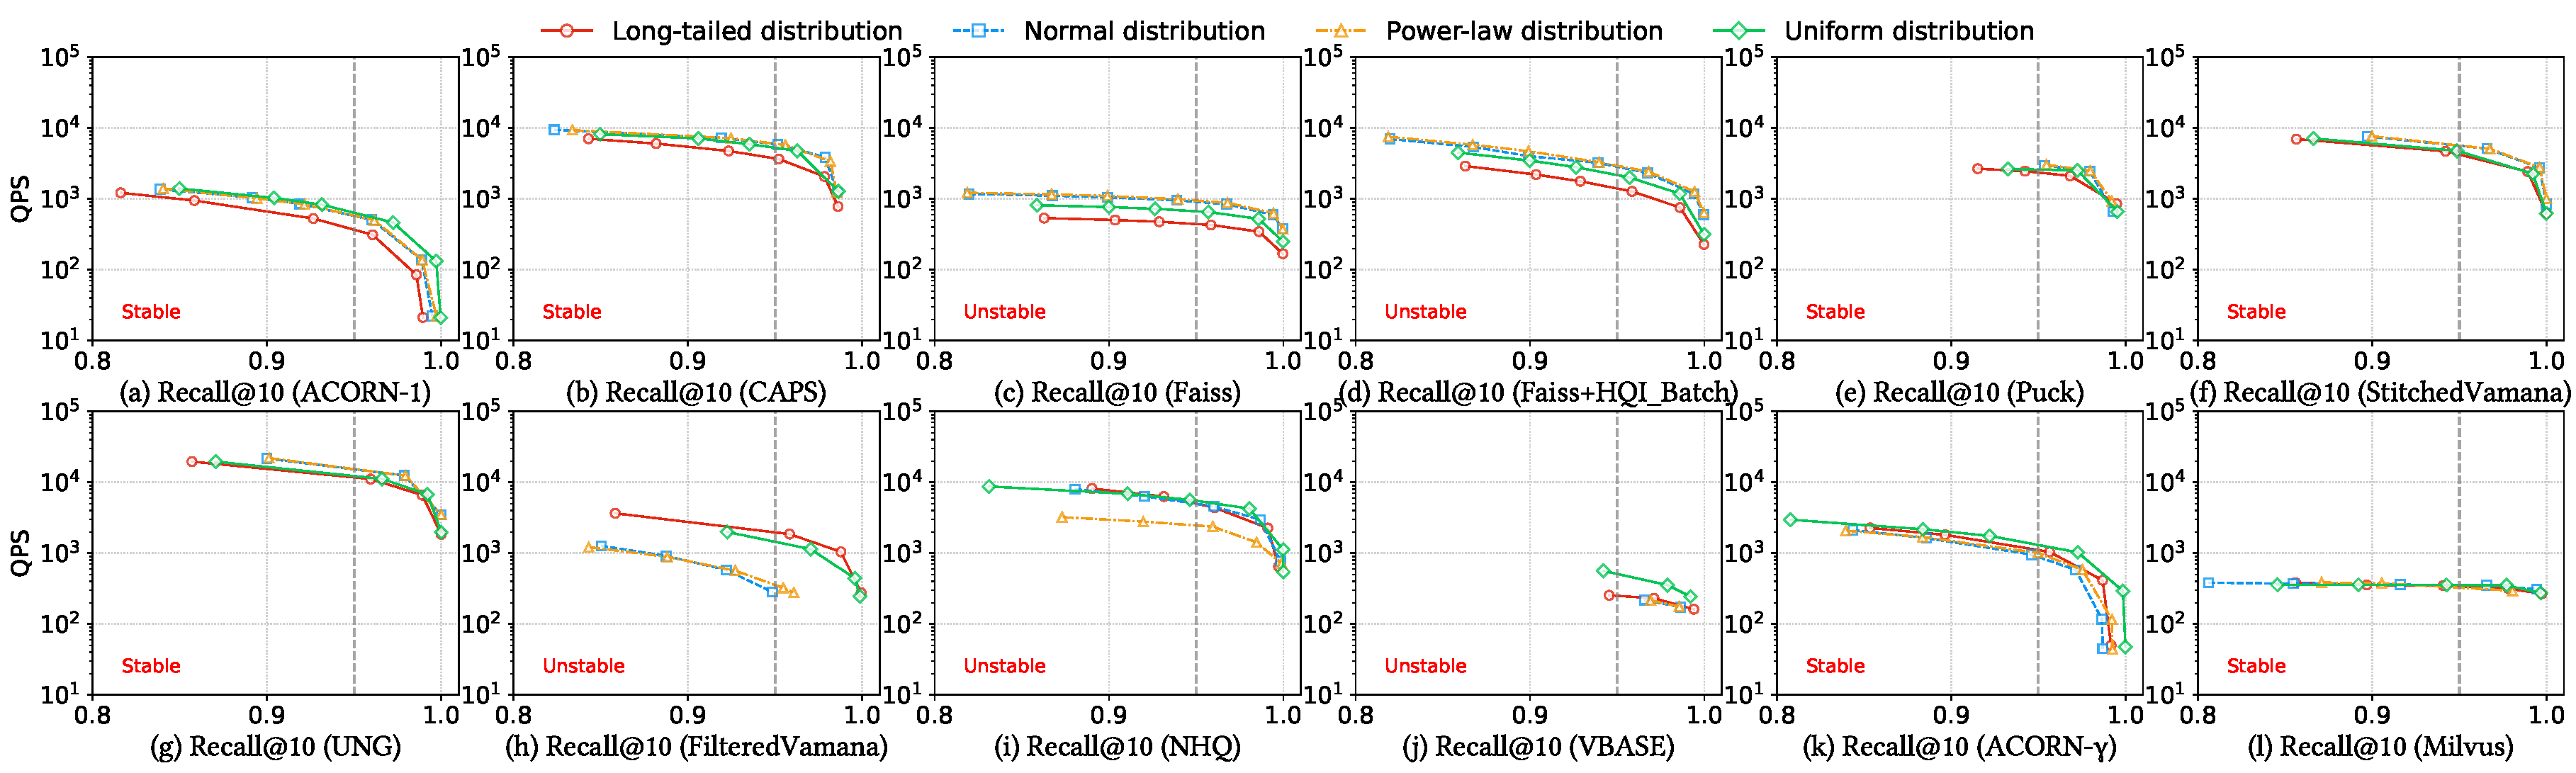
\includegraphics[width=0.95\textwidth]{figures/exp/exp_3_1.pdf}
	\caption{
		Effect of Attribute Distribution on Query Performance}
%		(Strong is robust to attribute distribution shifts, Weak is sensitive to attribute distribution shifts.)}
		
	\label{fig:exp_3_1}

%	\footnotesize{
%	\begin{center}
%			\begin{minipage}{\linewidth}
%				\centering	
%				\textit{Strong} : robust to attribute distribution shifts,  \textit{Weak} : sensitive to attribute distribution shifts
%			\end{minipage}
%	\end{center}
%	}
	\end{figure*}
	
	
	
	
	
	\textit{\textbf{Multi-Attribute Index Construction and Multi-Attribute Query.}}  
	Compared to single-attribute filtering, multi-attribute joint filtering better reflects real-world scenarios. To evaluate algorithm performance under this setting, we construct the index using 3 uniformly distributed attributes and apply filtering on all 3 attributes simultaneously during queries. \textcolor{black}{In this experiment, we only evaluate algorithms that support this multi-attribute query scenario.}
	
	As shown in Figure~\ref{fig:exp_4_1_MultiLabel_1thread}, UNG still maintains the best performance across all datasets. Since some strong competing algorithms do not support multi-attribute querying, CAPS becomes the second-best algorithm, but its performance on small datasets is relatively poor. This is because CAPS performs multi-level partitioning based on attributes on top of the IVF index, which introduces additional overhead. While this overhead negatively impacts performance on small datasets, on large datasets, the overhead is amortized, and the increasing dataset scale makes the advantages of attribute-aware partitioning evident.
	
	NHQ performs moderately overall in multi-attribute joint filtering scenarios but poorly on small datasets. Its reliance on fusion distance computations makes it highly sensitive to the number of attributes, impacting both efficiency and accuracy under multi-attribute filtering.
	For IVF-based methods not specifically optimized for hybrid queries (Faiss and Milvus), their QPS shows a similar and relatively stable trend as recall varies. Among them, Milvus, as a general-purpose system, exhibits comparatively poor performance.
	
	
	
	
	
	\subsubsection{Robustness}In the following, we evaluate the robustness of these algorithms.
	
	\textit{\textbf{Attribute Distribution.}} To evaluate the impact of attribute distribution, we generate base and query attributes \textcolor{black}{on the SIFT dataset using four representative distributions: long-tail, normal, power-law, and uniform.}
%	with four representative distributions—long-tail, normal, power-law, and uniform—across six datasets. 
%	Since performance differences across datasets are small, we report results on SIFT1M due to space limits.
	As illustrated in Figure~\ref{fig:exp_3_1}, the evaluated algorithms exhibit varying degrees of sensitivity to attribute distribution shifts. PASE is excluded due to poor past performance. \textcolor{black}{The proximity of the curves in the figure reflects algorithm sensitivity to attribute distributional variations. When the curves converge closely, it demonstrates that the algorithm maintains stable performance when attribute distributions change.} 
%	Specifically, ACORN, Milvus, Puck, CAPS, StitchedVamana, and UNG demonstrate strong robustness to such shifts. In contrast, Faiss, FilteredVamana, NHQ, VBASE, and PASE show notable sensitivity.


	Algorithms that are highly sensitive to attribute distribution tend to rely passively on the statistical characteristics of the attributes in their design. For instance, graph-based indexing methods like FilteredVamana and NHQ are prone to degraded connectivity or distorted structures under power-law distributions, where label frequencies are highly imbalanced. Similarly, VBASE, which employs a post-filtering strategy, shows efficiency that directly correlates with attribute selectivity—the more selective the filter, the more computational resources are wasted on retrieving irrelevant vectors. Faiss, which searches within the nearest clusters, may need to traverse more clusters to find sufficient results when relevant data points are unevenly distributed across clusters due to attribute skew, which impacts performance.

	In contrast, algorithms with low sensitivity to attribute distribution incorporate smarter indexing designs or adaptive query strategies to mitigate these challenges. Milvus, for example, leverages a built-in query optimizer that dynamically determines whether to filter by attributes or search vectors first, based on the selectivity of the query, thus ensuring more robust performance. Other approaches enhance robustness by separating attribute and vector indexing into distinct stages: UNG uses a logical graph to navigate attribute relationships, while CAPS employs an attribute frequency tree to adapt to power-law patterns. For ACORN--\(\gamma\), during index construction, attributes are primarily used for pruning in the lowest-layer graph, while the upper-layer hierarchical navigation graphs remain largely unaffected. Consequently, changes in attribute distribution have minimal impact on overall performance.
		

	
	\textit{\textbf{Single-Attribute Selectivity.}}
	In hybrid queries, varying attribute selectivity (AS) can significantly impact computational cost and query efficiency.
%	, as the algorithm must efficiently identify data points matching specific attributes within large datasets. 
	AS is defined as the proportion of data points sharing a given attribute value. For example, AS of 1\% indicates that only 1\% of the dataset meets the given attribute. 
	To investigate this effect, we evaluate 4 AS settings (1\%, 25\%, 50\%, and 75\%) on the SIFT1M dataset. 
%	We compare the query performance of attribute filtering algorithms across these settings, as shown in Figure~\ref{fig:exp_5_1_1_SingleLabel_1thread}.
	Based on the query performance trends of different algorithms under varying AS, we categorize the algorithms into 3 groups:

	
	
	\begin{figure*}
		\centering
		
		% 第一行:单独一张大图
		\begin{subfigure}{\textwidth}
			\centering
			
			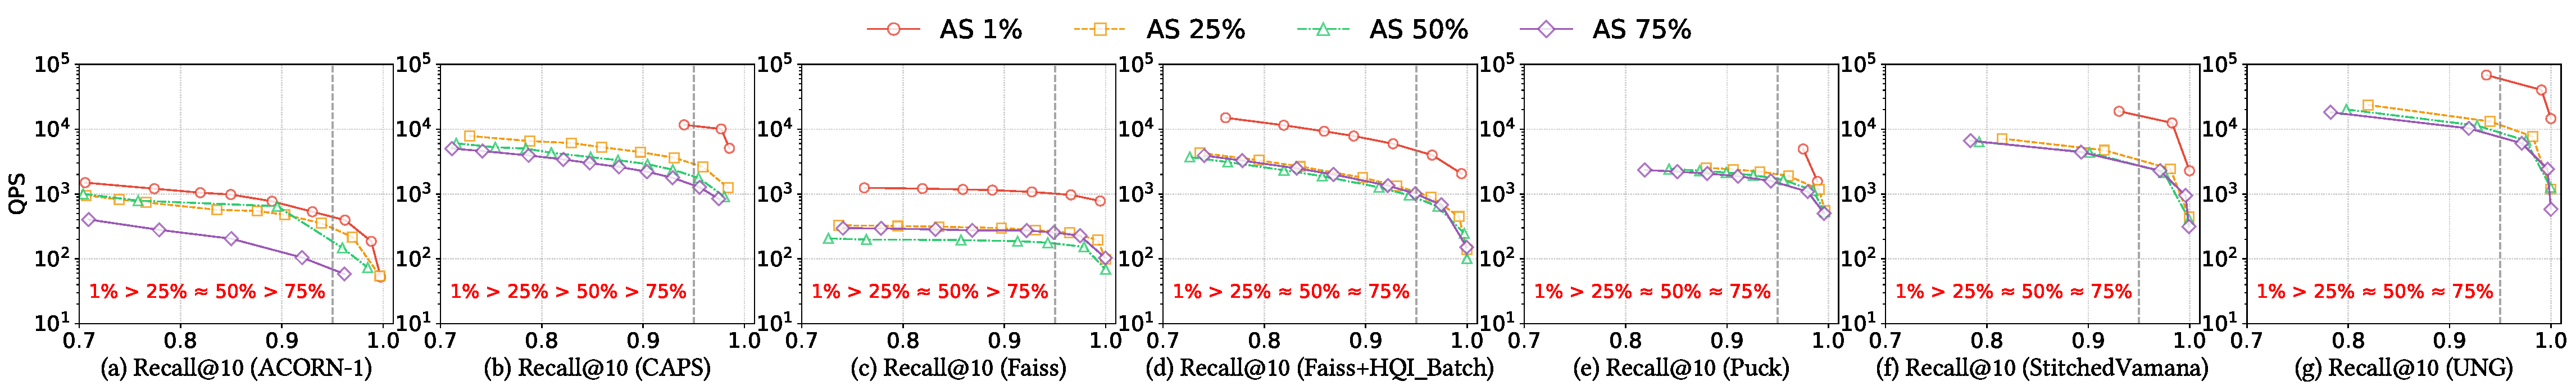
\includegraphics[width=0.98\textwidth]{figures/exp/exp_5_2_1.pdf}
			\caption{Algorithms Optimized for Low AS}
			\label{fig:exp_5_2_1}
		\end{subfigure}
		
		\vfill % 增加垂直间距
		
		% 第二行:两张子图,左侧宽度是右侧的两倍
		\begin{subfigure}{0.64\textwidth} % 2/3 宽度
			\centering
			
			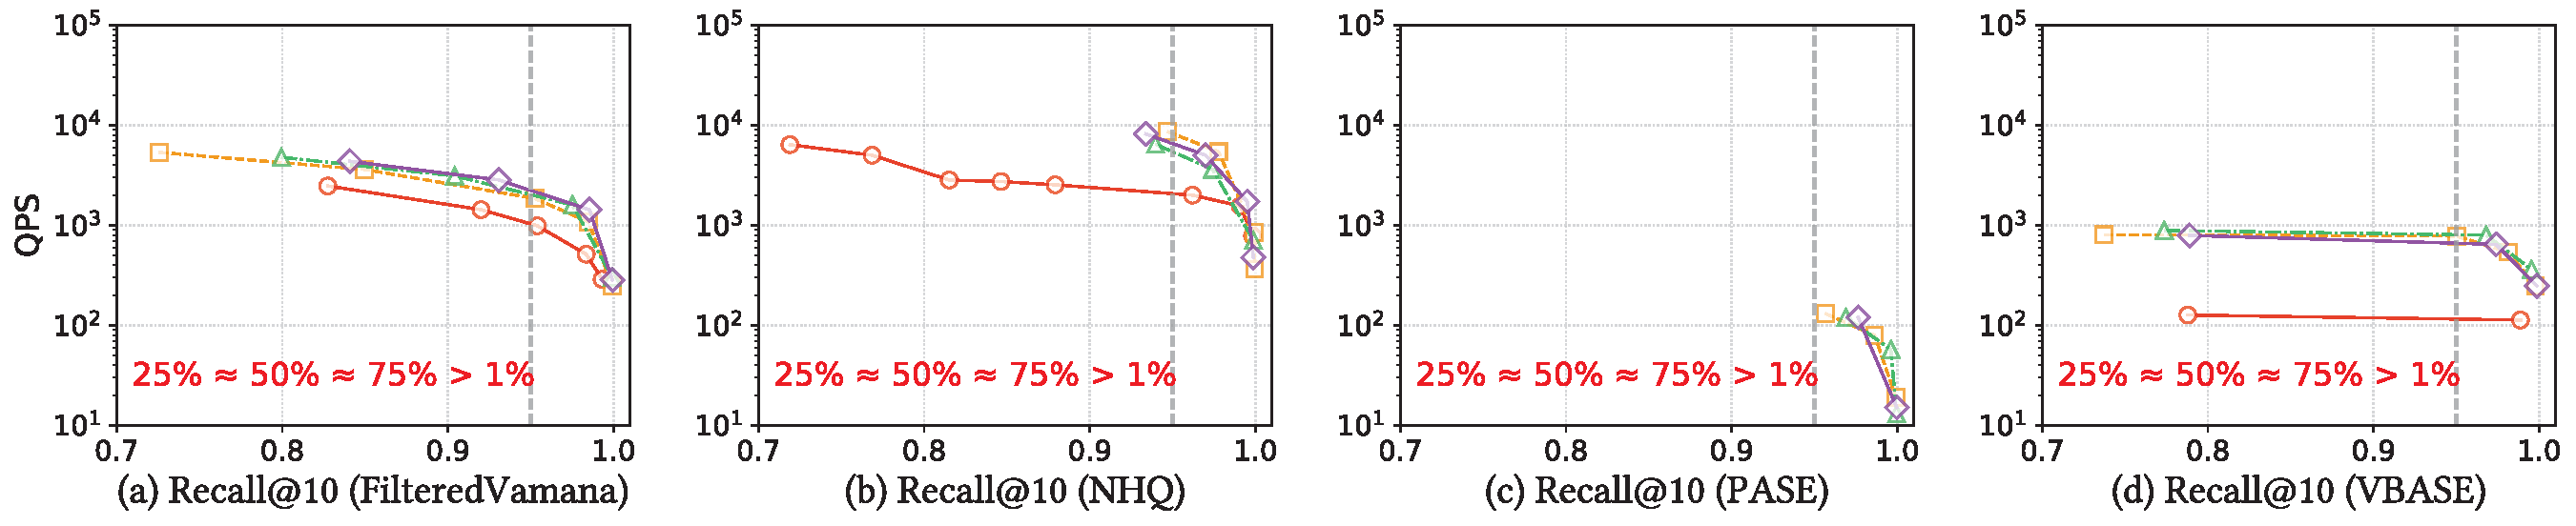
\includegraphics[width=0.96\textwidth]{figures/exp/exp_5_2_2.pdf}
			\caption{Algorithms Optimized for High AS}
			\label{fig:exp_5_2_2}
		\end{subfigure}
		\hspace{1mm} % 增加水平间距
		\begin{subfigure}{0.34\textwidth} % 1/3 宽度
			\centering
			
			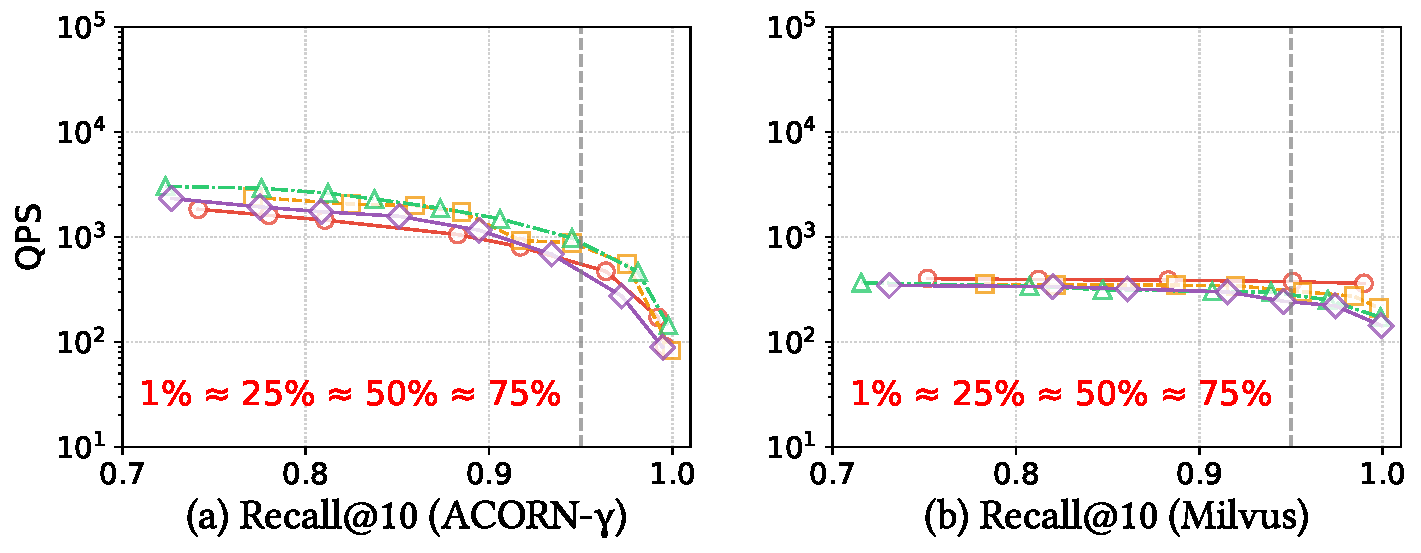
\includegraphics[width=0.96\textwidth]{figures/exp/exp_5_2_3.pdf}
			\caption{Algorithms Insensitive to AS}
			\label{fig:exp_5_2_3}
		\end{subfigure}
		
		\setlength{\abovecaptionskip}{0.15cm}
		\setlength{\belowcaptionskip}{-0.10cm}
		
		\caption{Performance of Different Attribute Selectivity (AS) under the Same Algorithm}
		\label{fig:exp_5_2_combined}
	\end{figure*}
	
	
	
	
	(1) \textit{Algorithms optimized for low AS.}  
%	This group includes ACORN-1, CAPS, Faiss, Faiss+HQI\_Batch, Puck, StitchedVamana and UNG, as illustrated in Figure~\ref{fig:exp_5_2_1}.
	\textcolor{black}{Figure~\ref{fig:exp_5_2_1} shows the algorithms suitable for low AS.}
	\textcolor{black}{ACORN-1}, Faiss, Puck, and UNG all use pre-filtering strategies to shrink the search space in low AS, leading to better performance. \textcolor{black}{Pre-filtering strategies significantly reduce the number of candidate points under low AS, thereby lowering the cost of  computations. As a result, such strategies tend to perform better in low AS scenarios.} CAPS efficiently skips irrelevant subpartitions, reducing computational overhead. However, as AS increases, it must process more subpartitions and handle a larger dataset. StitchedVamana optimizes local adjacency using independent subgraphs, enabling fast localization at low AS. However, at higher AS, it requires broader global exploration. 
	

	
	\par
	(2) \textit{Algorithms optimized for high AS.}  
%	This group includes FilteredVamana, NHQ, PASE and VBASE, as shown in Figure~\ref{fig:exp_5_2_2}.
	\textcolor{black}{Figure~\ref{fig:exp_5_2_2} shows the algorithms suitable for high AS.}
	At low AS, FilteredVamana performs poorly in these scenarios. Its dynamic pruning strategy makes it difficult to balance vector distance and attribute relevance, resulting in overly restricted search paths. NHQ struggles to locate relevant regions efficiently, leading to excessive computations on non-matching nodes. 
	 PASE performs poorly at extremely low AS (e.g., 1\%), with recall dropping below 0.2. Its fixed candidate set may not contain enough valid results after filtering, leading to incomplete top-$k$ results and significantly reducing recall. VBASE relies on post-filtering, which increases computational overhead at low AS.
	
	\par
	(3) \textit{Algorithms insensitive to AS.}  
%	This group includes Milvus and ACORN-\(\gamma\), as illustrated in Figure~\ref{fig:exp_5_2_3}.
	\textcolor{black}{Figure~\ref{fig:exp_5_2_3} shows algorithms that are insensitive to AS.}
	Milvus is mainly limited by system-level communication overhead, such as API latency. As a result, its query performance remains largely unaffected by AS variations. ACORN-\(\gamma\) maintains stable performance across different AS settings by using a higher index construction parameter $\gamma$. This ensures a relatively stable average node degree, even after attribute pruning, minimizing the impact of AS changes on query efficiency.
	


\begin{figure*}
	\centering
	
	
\includegraphics[width=0.9\textwidth]{figures/exp/attribute_legend.pdf}
	
	\begin{minipage}[t]{0.36\textwidth}
		\centering
		
		% 内部图片宽度使用\linewidth,它会自适应为容器宽度(0.32\textwidth)
		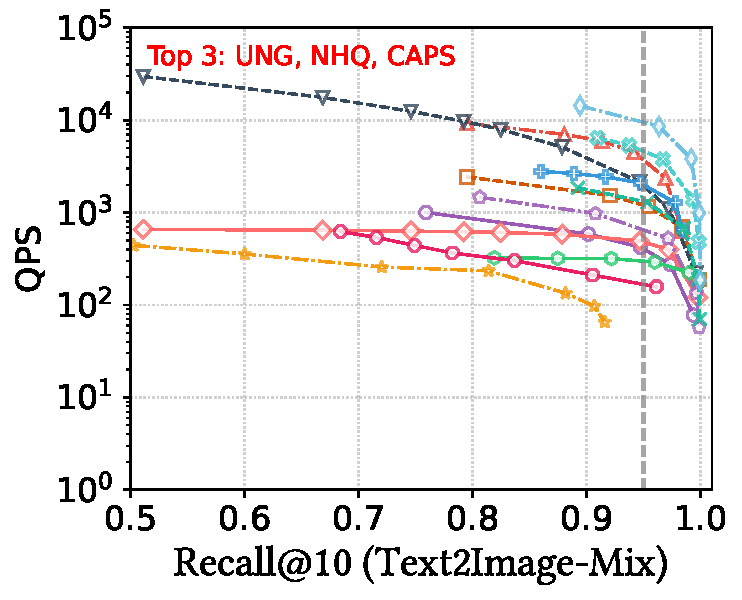
\includegraphics[width=0.495\linewidth]{figures/exp/attribute_multimodel.pdf}
		\hfill 
		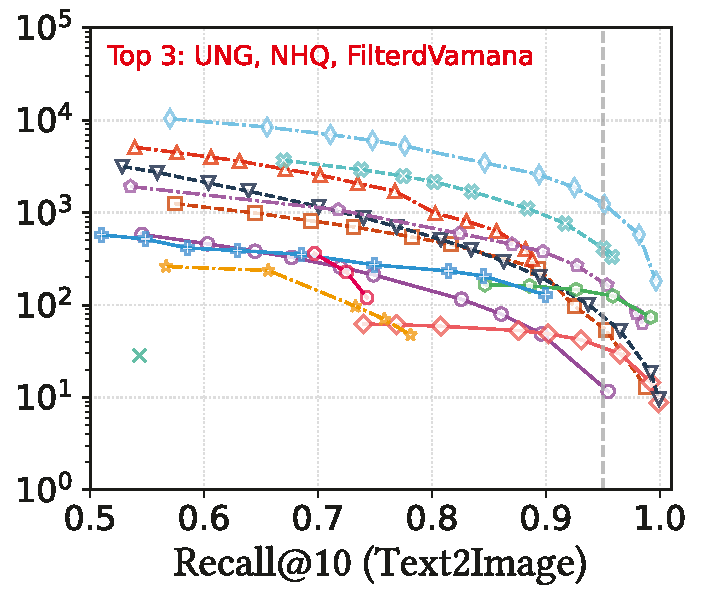
\includegraphics[width=0.47\linewidth]{figures/exp/attribute_multimodel_1.pdf}
		
	\end{minipage}
	\hfill
	\begin{minipage}[t]{0.20\textwidth}
		\centering
		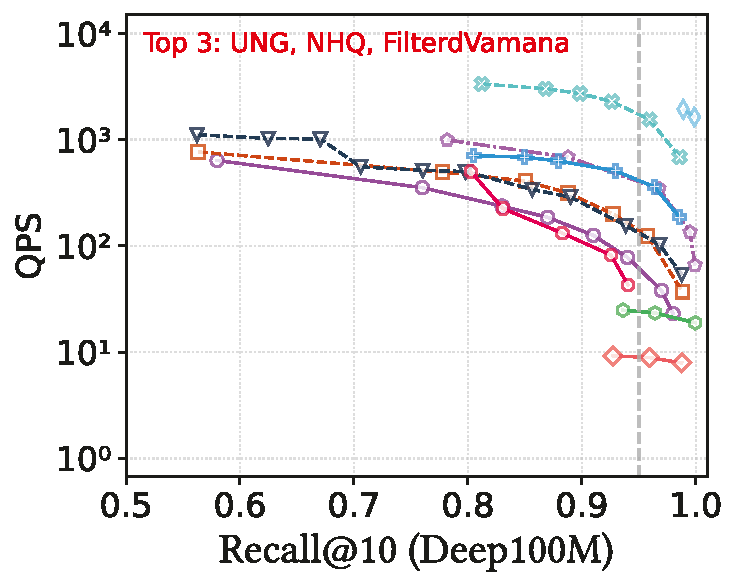
\includegraphics[width=0.9\linewidth]{figures/exp/attribute_100M.pdf} 
		
	\end{minipage}
	\hfill % 在盒子之间添加弹性间距
	\begin{minipage}[t]{0.37\textwidth}
		\centering
		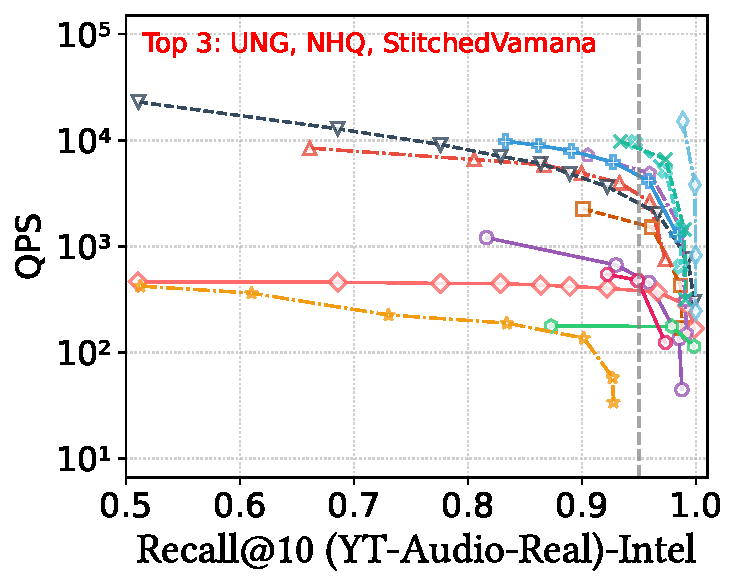
\includegraphics[width=0.495\linewidth]{figures/exp/attribute_85.pdf}
		\hfill
		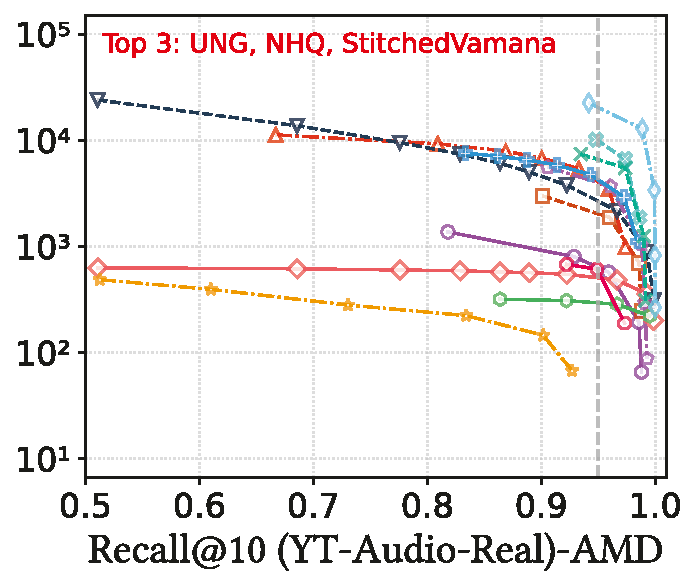
\includegraphics[width=0.47\linewidth]{figures/exp/attribute_71.pdf}
		
	\end{minipage}

\end{figure*}


\begin{figure*}
	\centering
%	\setlength{\abovecaptionskip}{0.0cm}
	\begin{minipage}[t]{0.37\textwidth}
		\centering
		\setlength{\abovecaptionskip}{-0.2cm}
		\setlength{\belowcaptionskip}{-0.25cm}
		\caption{Multi-Modal Datasets (AF)}
		\label{fig:attribute-multimodal}  
	\end{minipage}%
	\hfill
	\begin{minipage}[t]{0.27\textwidth}
		\centering
		\setlength{\abovecaptionskip}{-0.2cm}
		\setlength{\belowcaptionskip}{-0.25cm}
		\caption{Large-Scale Dataset (AF)}
		\label{fig:attribute big dataset}
	\end{minipage}
	\hfill 
	\begin{minipage}[t]{0.35\textwidth}
		\centering
		\setlength{\abovecaptionskip}{-0.2cm}
		\setlength{\belowcaptionskip}{-0.25cm}
		\caption{Different Platforms (AF)}
		\label{fig:attribute-cross-platform}
	\end{minipage}%
\end{figure*}
	


%	\subsubsection{Scalability Study}
	\textit{\textbf{\textcolor{black}{Multi-Modal Queries.}}} \textcolor{black}{
	We conduct experiments on two multi-modal  datasets Text2image-Mix and Text2image. 
%This dataset contains image and text vectors and is a hybrid multi-modal dataset. 
On Text2image-Mix dataset, as shown in Figure~\ref{fig:attribute-multimodal}, UNG and NHQ consistently perform best, followed by CAPS.
Although the dataset contains two modalities, due to the significant differences between the modalities, they are actually two separate regions in the vector space. The performance is similar to that of the single-modal dataset in Figure~\ref{fig:exp_1_1_SingleLabel_1thread}. This is because mixed multi-modal queries are actually the same as conducting experiments on two datasets of the same modality. This is not actually a difficult query.
%		Although this dataset mixes two modalities, the vector space distributions of different modalities often differ significantly. In practice, this means that the experiments effectively treat the image and text subsets as separate datasets, since the ground truths for each query belong to the same modality. Therefore, the performance on this dataset is similar to the results shown in Figure~\ref{fig:exp_1_1_SingleLabel_1thread}.
		In contrast, the Text2image dataset shown in Figure~\ref{fig:attribute-multimodal} is different. The query set and the base dataset belong to two completely different modalities. Queries are far from the dataset points, and the ground truths are more dispersed. To find the ground truths, algorithms typically need to examine more points, which leads to degraded performance.
	}
	
	\textit{\textbf{\textcolor{black}{Large-scale Dataset.}}} 
	\textcolor{black}{As shown in the Figure~\ref{fig:attribute big dataset}, on the Deep100M dataset, UNG and NHQ still exhibit excellent performance, demonstrating good adaptability to large-scale datasets. However, this also comes with significant memory overhead. The clustering-based algorithm Faiss+HQI\_Batch shows moderate performance but has very low memory overhead, which also has certain practical significance. Furthermore, we do not present the results of StitchedVamana and CAPS, as their recall remained consistently low. StitchedVamana sets the search entry point to 0 by default, which makes it prone to getting stuck in local optima when the entry is far from the target region, hindering effective navigation. CAPS, on the other hand, cannot properly run large-scale dataset experiments because its code implementation does not account for such scenarios.}
	
	\textit{\textbf{\textcolor{black}{Different Hardware Environments.}}} 
%	\textcolor{cyan}{To investigate the impact of different server configurations on the performance of the algorithms, we conducted additional experiments on Server B using the YT-Audio-Real dataset, and the results are shown in Figure~\ref{fig:Different Computer}. Compared with the experimental results on Server A shown in Figure~\ref{fig:exp_1_1_SingleLabel_1thread}f, the relative ranking of the algorithms remains largely unchanged, indicating that the performance of these methods is not significantly affected by differences in CPU configurations. Due to the lower CPU frequency and smaller RAM capacity of Server B compared to Server A, the QPS values are slightly lower across all methods.}
	\textcolor{black}{To investigate the impact of different server configurations on the performance of the algorithms, we conduct additional experiments on an Ubuntu 20.04 server equipped with dual Intel(R) Xeon(R) Gold 6330 CPUs @ 2.00GHz featuring 128GB of RAM and 84 MiB of L3 cache using the YT-Audio-Real dataset, and the results are shown in Figure~\ref{fig:attribute-cross-platform}. It is not difficult to see that the relative ranking of the algorithms under the two servers essentially remains unchanged, indicating that the performance of these methods is not significantly affected by differences in CPU configurations. Due to the lower CPU frequency, reduced RAM capacity, and smaller L3 cache, all methods demonstrate slightly lower QPS values.}

	



	\begin{figure}[t]
		\centering
		
		
		\hspace*{5pt}
		% 放大的图例(占满单栏)
		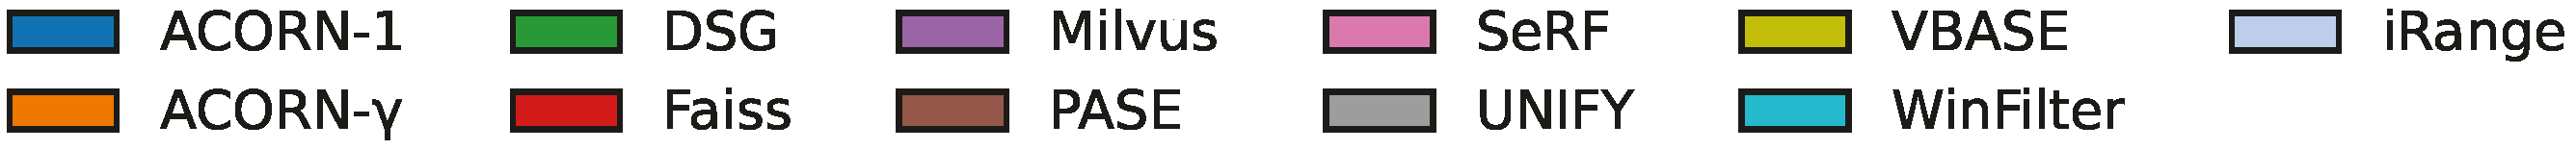
\includegraphics[width=0.98\columnwidth]{figures/indexData/rangeFilter_legend_only.png}
		
	
		
		% 三图横排
		\begin{subfigure}[t]{0.495\columnwidth}
			\centering
			\captionsetup{font=small}
			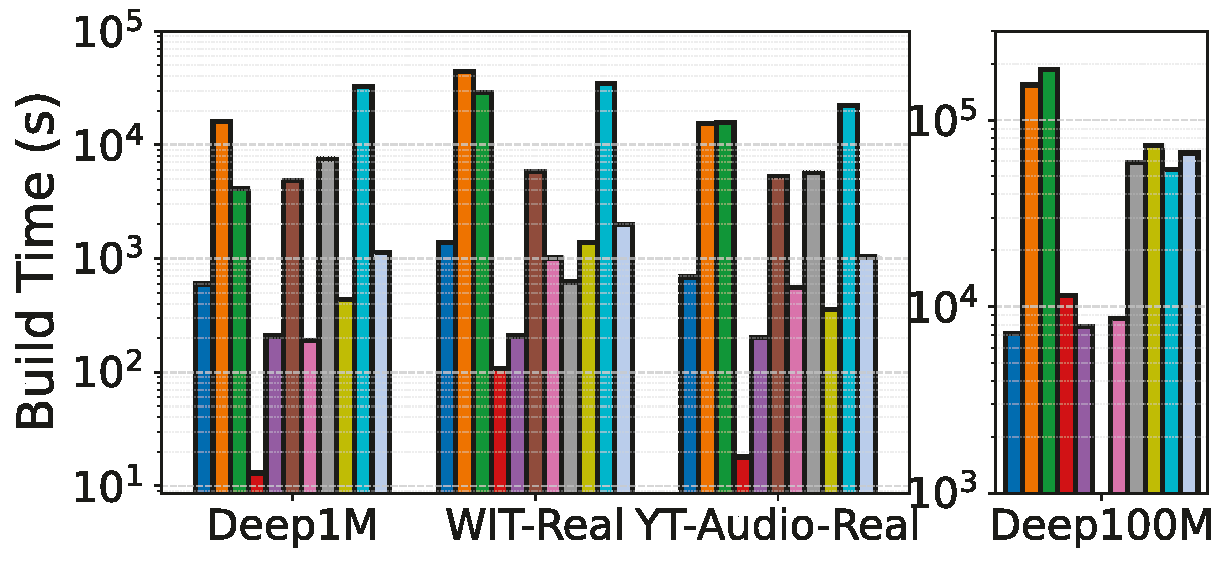
\includegraphics[width=\linewidth]{figures/indexData/rangeFilter_build_time_comparison_query.pdf}
			\caption{\footnotesize Construction Time}
			\label{fig:rangeFilter_build_time}
		\end{subfigure}
		\hfill
		\begin{subfigure}[t]{0.495\columnwidth}
			\centering
			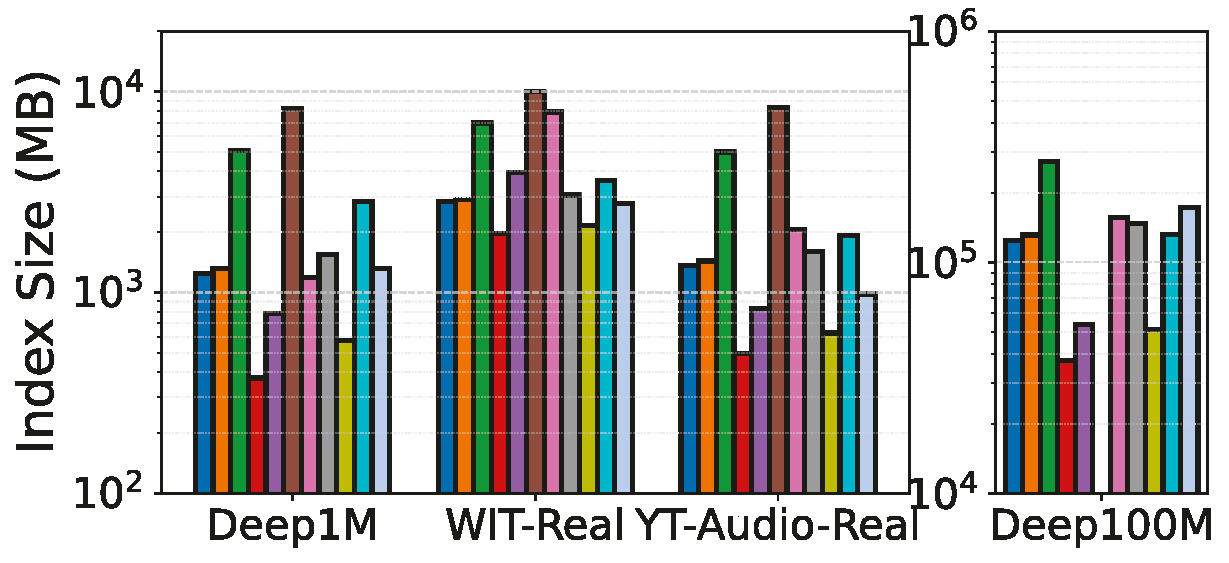
\includegraphics[width=\linewidth]{figures/indexData/rangeFilter_index_size_mb_comparison_query.pdf}
			\caption{\footnotesize Index Size}
			\label{fig:rangeFilter_index_size_mb}
		\end{subfigure}
		\hfill
		\begin{subfigure}[t]{0.495\columnwidth}
			\centering
			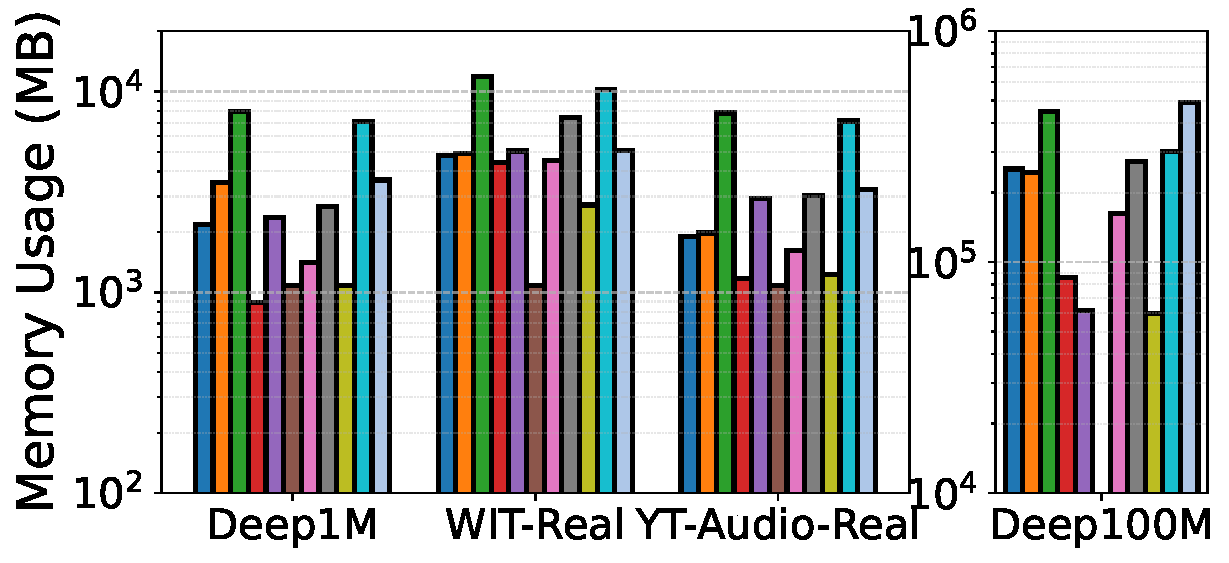
\includegraphics[width=\linewidth]{figures/indexData/rangeFilter_memory_mb_comparison_query.pdf}
			\caption{\footnotesize Build Peak Memory}
			\label{fig:rangeFilter_build_memory_mb}
		\end{subfigure}
		\hfill
		\begin{subfigure}[t]{0.495\columnwidth}
			\centering
			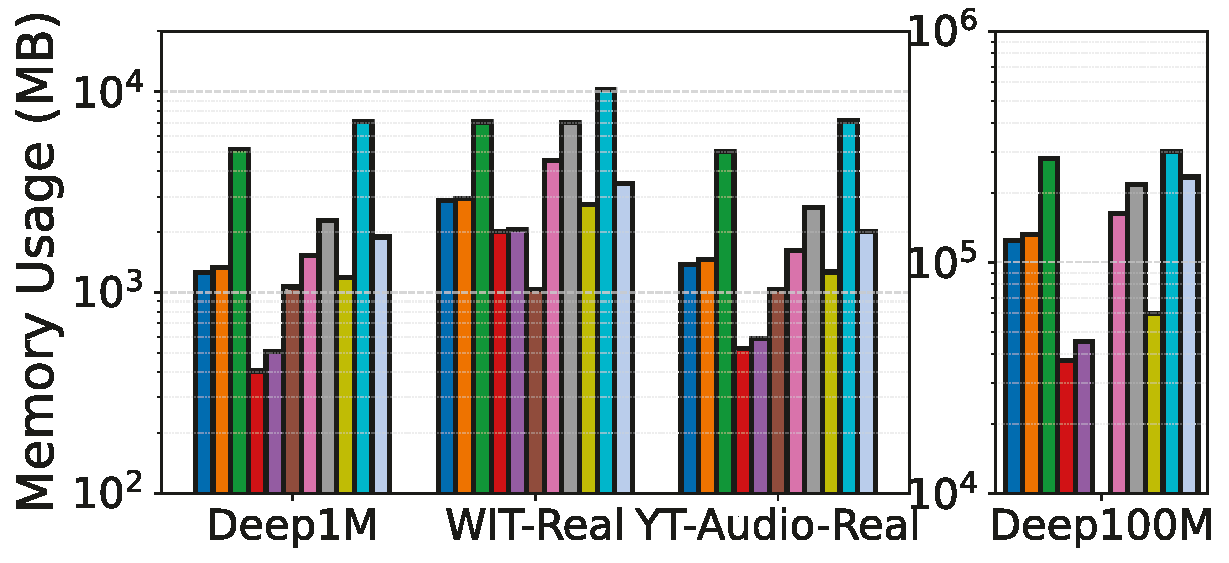
\includegraphics[width=\linewidth]{figures/searchMem/range_memory_comparison.pdf}
			\caption{\footnotesize Search Peak Memory}
			\label{fig:rangeFilter_search_memory_mb}
		\end{subfigure}
		
		%		\caption{Time and space overhead of range filtering index construction}
%		\caption{Time and space overhead of index construction}
		\setlength{\abovecaptionskip}{0.1cm}
		\setlength{\belowcaptionskip}{-0.3cm}
		\caption{\textcolor{black}{Time and Space Overhead (RF)}}
		\label{fig:rangeFilter_build_index_comparison}
	\end{figure}
	\subsection{Range Filtering}
	\textcolor{black}{Due to the limitations of existing range filtering algorithms, our experiment uses only a single attribute, with the dataset sorted in ascending order by value. The WIT-Real and YT-Audio-Real datasets use real attribute values, while the rest use randomly generated ones. }
	\subsubsection{\textcolor{black}{Time and Space overhead.}}
	
	%Similar to the evaluation of \textit{Attribute Filtering} algorithms, 
	Similarly, we also evaluate \textcolor{black}{4} key metrics mentioned above in \textit{Range Filtering} algorithms. \textcolor{black}{Notably, all algorithms use single-threaded index construction on medium-scale datasets, and 64-thread construction on the large-scale Deep100M dataset, except DSG, which only supports single-threading. For WinFilter, we use its integrated Super-Postfiltering on medium datasets for best performance, and switch to its base algorithm Vamana-WST on Deep100M due to construction overhead.
	}
	
	\textit{\textbf{Index construction time.}}
	\textcolor{black}{
	As shown in Figure~\ref{fig:rangeFilter_build_time}, Faiss and Milvus, based on the IVF architecture, require less time. This indexing structure enables fast construction through subset sampling and centroid computation, thereby reducing computational cost. Milvus performs particularly well on large-scale datasets, mainly due to its cache-aware optimizations, which significantly reduce CPU cache misses.}



\textcolor{black}{In addition, the two HNSW-based methods, ACORN-1 and SeRF, also achieve short index construction time. ACORN-1 closely follows the original HNSW construction process and reduces the number of candidate neighbors in the upper layers to lower computational overhead. SeRF attaches timestamp information to edges during construction, making the total build time comparable to that of a single HNSW graph.
	}



\textcolor{black}{We observe that ACORN-\(\gamma\), DSG and WinFilter exhibit relatively long index construction time. Although the first two methods are also based on HNSW, ACORN-\(\gamma\) extends the neighbor list of each node to provide more candidate paths, which increases both computational and memory overhead. DSG, on the other hand, incorporates a rectangle tree structure for index management, making the construction process more complex and costly. 
WinFilter also incurs high construction cost, as it relies on a tree structure and builds a separate nearest neighbor graph for each node, which leads to redundant computations. However, on large-scale datasets, its preprocessing stage is replaced by the base algorithm Vamana-WST, effectively avoiding significant time overhead.}





	
	


	
	\textit{\textbf{Index size.}} 
	As shown in Figure~\ref{fig:rangeFilter_index_size_mb}, Among all algorithms, Faiss has the smallest index size. Because IVF only adds centroid data and partition information to the vector dataset, the IVF index is only slightly larger than the vector dataset.

	
	\textcolor{black}{Similar to attribute filtering, PASE requires the most storage. }
	\textcolor{black}{Additionally, DSG also results in a large index size, especially on large-scale datasets. As an enhancement over SeRF, DSG stores additional metadata for each edge in its index structure. While this design improves retrieval accuracy, it significantly increases the index size on massive datasets.}


	

	
	\textcolor{black}{\textit{\textbf{Peak memory.}}  
	As explained in the attribute filtering analysis, methods with larger index sizes (including the dataset) tend to exhibit higher peak memory consumption. As shown in Figure~\ref{fig:rangeFilter_build_memory_mb} and Figure~\ref{fig:rangeFilter_search_memory_mb}, range filtering also adheres to this pattern.}  
%	, while PASE deviates due to reasons discussed earlier

	\textcolor{black}{WinFilter also presents an exception:  its peak memory usage is also affected by the level of parallelism. Although the final index size remains relatively small, the peak memory usage increases significantly during both construction and search. During construction, this is caused by the parallel building of local indices for each tree node, which results in substantial temporary memory usage. Similarly, during search, WinFilter needs to load multiple local indices in parallel for different tree nodes, further contributing to high peak memory consumption.}
	

	





		
	\begin{figure*}[t]
		
		\centering
		
		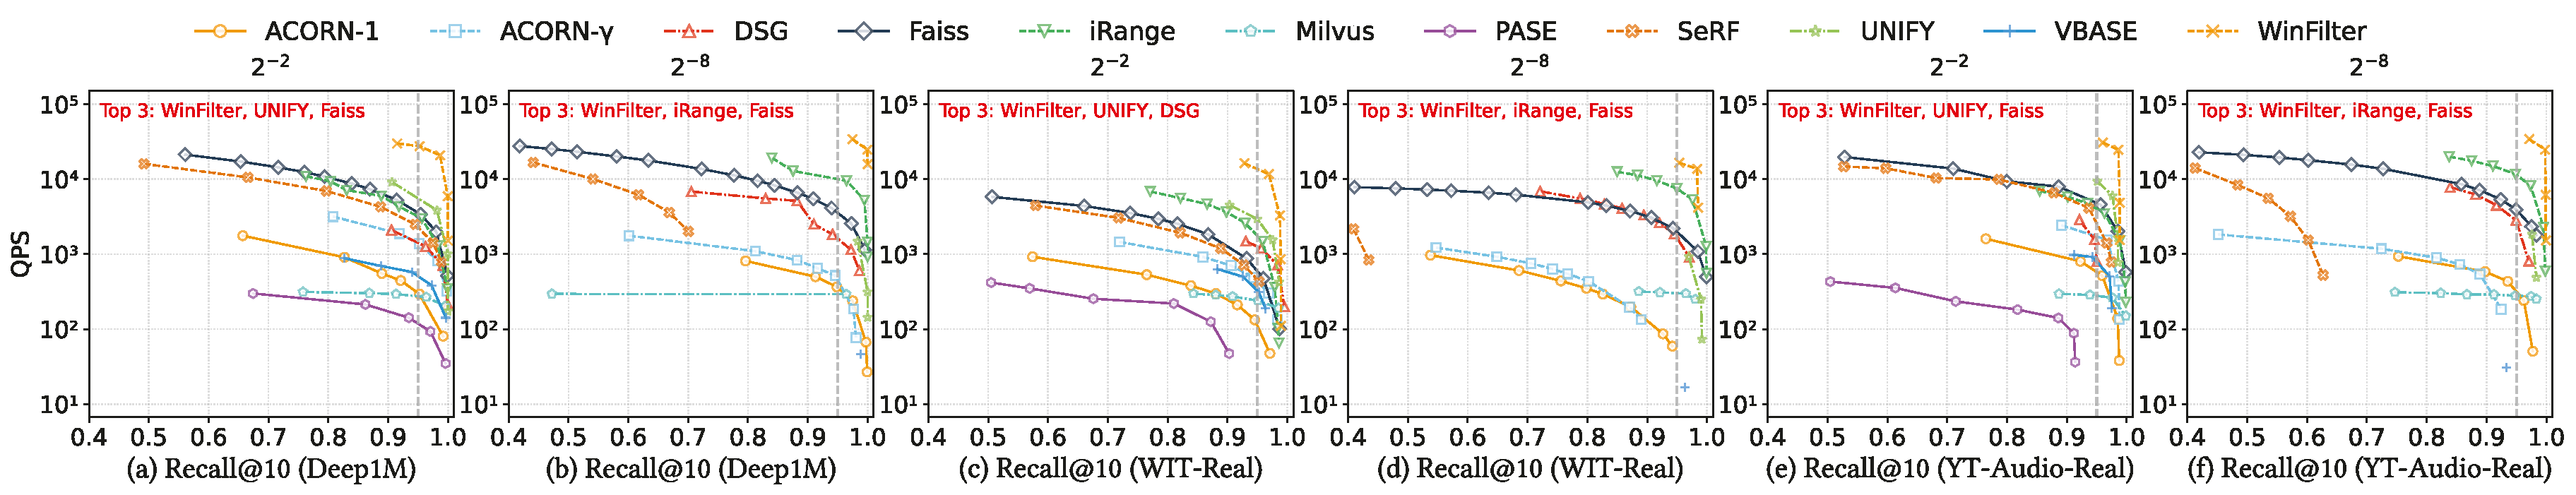
\includegraphics[width=0.99\textwidth]{figures/exp/exp_8_2.pdf}
		\setlength{\abovecaptionskip}{0.1cm}
		\setlength{\belowcaptionskip}{-0.15cm}
		\caption{Performance of RF-ANN Search}
		\label{fig:exp_8_2}
	\end{figure*}
	
	
	\subsubsection{Performance Evaluation. }
	
	In this experiment, we follow the query range definition adopted by prior work~\cite{HQI}. \textcolor{black}{Specifically, for a given query, the range ratio is defined as $2^{-i}$	when the query range covers $\frac{n}{2^i}$ data points, where $n$ is the total dataset size.}


	Based on this definition, we evaluate algorithm performance under four query range settings: $2^{-2}$, $2^{-4}$, $2^{-6}$, and $2^{-8}$. For space considerations, Figure~\ref{fig:exp_8_2} reports results for only the largest ($2^{-2}$) and smallest ($2^{-8}$) range ratios. 
%	The experimental results show consistent performance across all datasets and query ranges.
	

	
	\textcolor{black}{
		As shown in Figure~\ref{fig:exp_8_2}, the algorithms that performed well are WinFilter, iRange, UNIFY, and Faiss.
	WinFilter maintains optimal performance by building an index for each tree node. It then performs an ANN search on the relevant nodes and post-filters the results, ensuring high recall and QPS.
	In contrast, iRange dynamically constructs a search graph during querying. This method has low overhead and performs well in small-range queries, but its performance degrades as the query range increases.
	UNIFY utilizes a skip list for localization followed by a linear scan for searching in small-range query scenarios. Its performance is generally lower than graph-based structures like iRange in these cases.
	Interestingly, Faiss, aided by its efficient ID selector for filtering, calculates distances for only a small subset of points in small-range scenarios. Consequently, it can outperform algorithms specifically designed for range searches.
	}

	\textcolor{black}{SeRF, ACORN, and vector databases performed poorly.
		SeRF demonstrates relatively weak overall performance, with a pronounced drop in recall under small-range query scenarios. This is because SeRF compresses the entire HNSW graph by attaching range information to its edges. However, during small-range queries, its multi-filtering mechanism requires scanning a large number of edge entries that are irrelevant to the current query range, introducing fixed computational and memory access overhead. Additionally, graph traversal may lead to the exploration of numerous invalid neighbors, increasing the likelihood of the search becoming trapped in local optima and further degrading performance.
		The overall performance of ACORN is poor. Unlike other algorithms specifically designed for range filtering, ACORN does not design an index specifically for range queries. Instead, it adopts a pre-filtering strategy, resulting in poorer performance.
		The performance of vector databases is also poor in range queries, as they are not specifically optimized for such queries. PASE performs particularly poorly in small range queries, with a recall rate lower than 0.1, mainly due to its post-filtering strategy.
	}

	
	
	
	
\begin{figure*}
	\centering
	
\includegraphics[width=0.7\textwidth]{figures/exp/range_legend.pdf}
	
	\begin{minipage}[t]{0.36\textwidth}
		\centering
		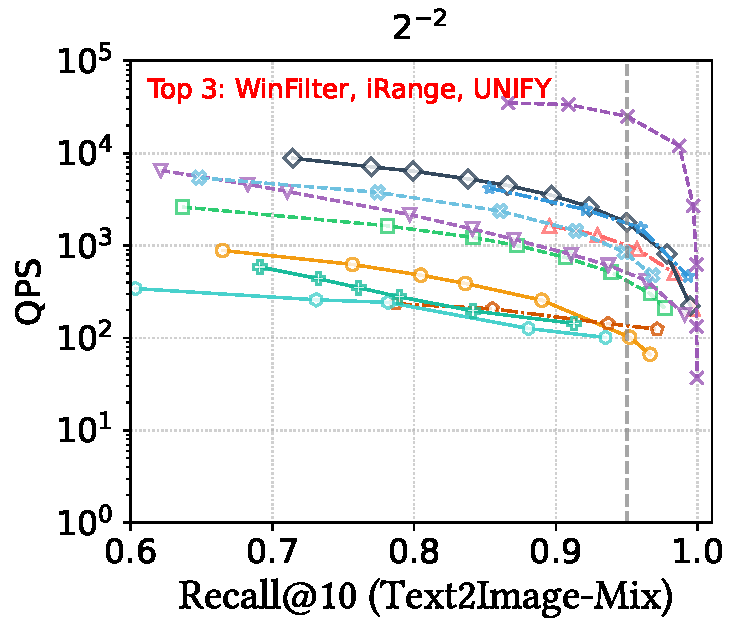
\includegraphics[width=0.495\linewidth]{figures/exp/range_multimodel.pdf}
		\hfill 
		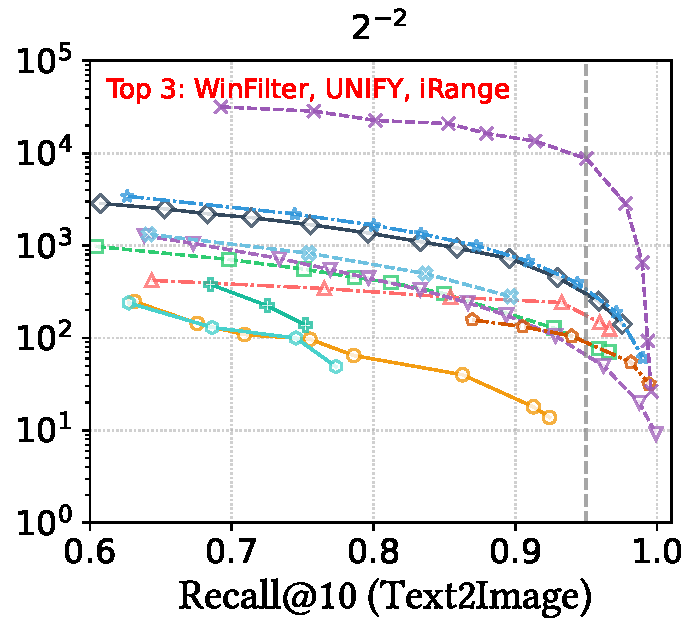
\includegraphics[width=0.47\linewidth]{figures/exp/range_multimodel_1.pdf}

	\end{minipage}
	\hfill
	\begin{minipage}[t]{0.18\textwidth}
		\centering
		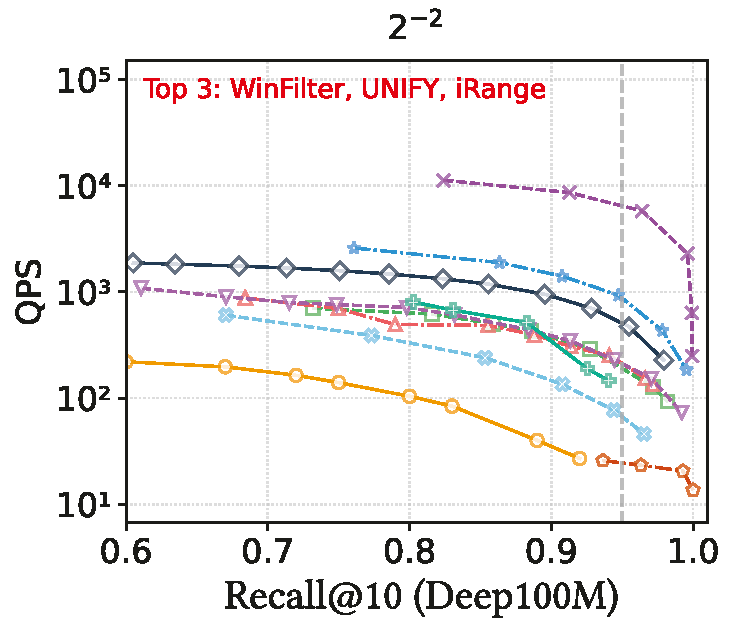
\includegraphics[width=0.96\linewidth]{figures/exp/range_deep100M.pdf} 
	\end{minipage}
	\hfill % 在盒子之间添加弹性间距
	\begin{minipage}[t]{0.36\textwidth}
		\centering
		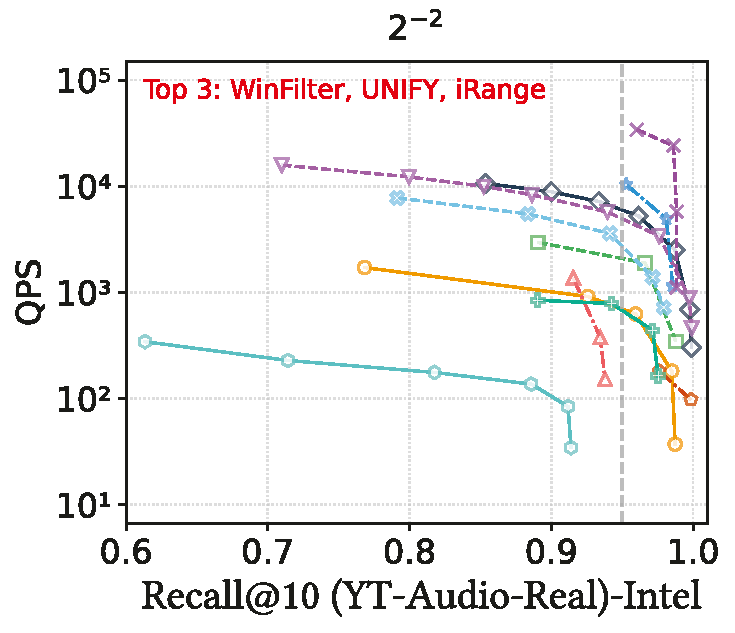
\includegraphics[width=0.495\linewidth]{figures/exp/range_85.pdf}
		\hfill
		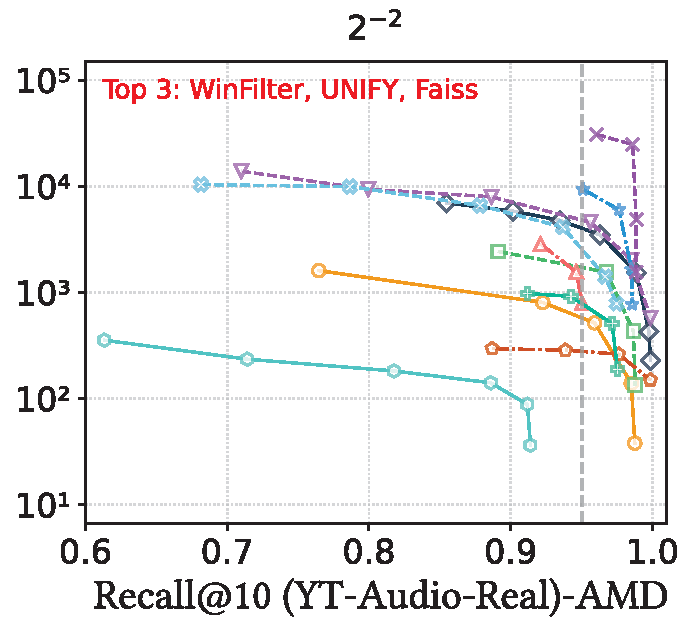
\includegraphics[width=0.47\linewidth]{figures/exp/range_71.pdf}
	\end{minipage}
\end{figure*}

\begin{figure*}
	\centering
	\begin{minipage}[t]{0.37\textwidth}
		\centering
		\setlength{\abovecaptionskip}{-0.2cm}
		\setlength{\belowcaptionskip}{-0.3cm}
		\caption{Multi-Modal Datasets (RF)}
		\label{fig:range-multimodal} 
	\end{minipage}%
	\hfill
	\begin{minipage}[t]{0.27\textwidth}
		\centering
		\setlength{\abovecaptionskip}{-0.2cm}
		\setlength{\belowcaptionskip}{-0.3cm}
		\caption{Large-Scale Dataset (RF)}
		\label{fig: range big dataset}
	\end{minipage}
	\hfill % 在盒子之间添加弹性间距
	\begin{minipage}[t]{0.35\textwidth}
		\centering
		\setlength{\abovecaptionskip}{-0.2cm}
		\setlength{\belowcaptionskip}{-0.3cm}
		\caption{Different Platforms (RF)}
		\label{fig:range-cross-platform}
	\end{minipage}%
	
\end{figure*}
	
	\subsubsection{Robustness}
	
	\textit{\textbf{\textcolor{black}{Multi-Modal Queries.}}}
	\textcolor{black}{
		Similar to attribute filtering, the performance of range filtering queries on the Text2image-Mix dataset (Figure~\ref{fig:range-multimodal}) is similar to the single-modality query performance (Figure~\ref{fig:exp_8_2}). However, on the Text2Image dataset, these algorithms exhibit a significant performance degradation (Figure~\ref{fig:range-multimodal}). This is because most of these range query algorithms are graph-based, and such algorithms require more iterations to find true neighbors in OOD datasets.
		}
		
	\textit{\textbf{\textcolor{black}{Large-scale Dataset.}}} \textcolor{black}{As shown in the Figure~\ref{fig: range big dataset}, On the Deep100M dataset, the top 3 ranked algorithms (WinFilter, UNIFY, and iRange) remain unchanged. However, their high performance is achieved at the cost of extremely high memory consumption (Figure~\ref{fig:rangeFilter_search_memory_mb}). In contrast, VBASE and Faiss demonstrate moderate performance while consuming significantly less memory.}
		
	\textit{\textbf{\textcolor{black}{Different Hardware Environments.}}} 
	\textcolor{black}{Consistent with Section 4.2.3, we conduct range filtering experiments on the YT-Audio-Real dataset using two server configurations, with results presented in Figure~\ref{fig:range-cross-platform}. Although the third-ranked algorithm differs, we consider the ranking order remains stable since the performance of the third and fourth algorithms is comparable. Therefore, different server configurations only affect the performance of individual algorithms, with minimal impact on their relative performance ranking.}  


	

	
	
%	\textit{\textbf{Multimodel, 85 and Deep100M.}} \textcolor{red}{The fig is Figure \ref{fig:TrinityExtension——Range}}
	\section{DISCUSSION}
	\textcolor{black}{Based on the performance of algorithms across various experimental settings, we evaluate their strengths and weaknesses in different application scenarios, as shown in Table \ref{tab:algorithm_recommendation}. Next, we provide a comprehensive discussion of the advantages and disadvantages of each algorithm.}
	
	
	
	\subsection{Recommendations.}
	%Based on the performance of different algorithms in experiments, we recommend algorithms suitable for different scenarios, as shown in the table \ref{tab:algo_scenarios}.
	
\begin{table*}[htbp]
	\setlength{\abovecaptionskip}{0.1cm}
	\setlength{\belowcaptionskip}{0.1cm}
	\caption{Algorithm Recommendation}
	\label{tab:algorithm_recommendation}
	\resizebox{\textwidth}{!}{
\large
\begin{tabular}{|l|*{16}{c|}}
	\hline
	\multirow{2}{*}{\textbf{Application Scenarios }} 
	& \multicolumn{6}{c|}{\textbf{AF}} 
	& \multicolumn{5}{c|}{\textbf{RF}} 
	& \multicolumn{5}{c|}{\textbf{AF / RF}} \\
	\cline{2-17}
	& \textbf{UNG} & \textbf{NHQ} & \textbf{Filtered} & \textbf{Stitched} & \textbf{CAPS} & \textbf{Puck} 
	& \textbf{Win} & \textbf{iRange} & \textbf{SeRF} & \textbf{DSG} & \textbf{UNIFY} 
	& \textbf{ACORN} & \textbf{Faiss} & \textbf{Milvus} & \textbf{VBASE} & \textbf{PASE} \\
	\hline
	\textbf{Performance-Critical} & \textbf{B} & G & M & G & M & G & G & M & M & M & M & M/M & M/M & M/M & P/P & P/P \\
	\hline
	\textbf{Index-Efficient} & M & M & M & M & M & G & P & M & G & P & P & P/P & \textbf{B}/\textbf{B} & G/G & P/M & P/P \\
	\hline
	\textbf{Memory-Constrained} & M & P & M & M & M & G & P & P & M & P & P & P/P & \textbf{B}/\textbf{B} & G/M & G/M & G/G \\
	\hline
	\textbf{Large-Scale} & \textbf{B} & G & G & P & P & G & \textbf{B} & G & M & M & G & M/P & P/M & P/P & M/M & - \\
	\hline
%	\textbf{Multi-Modal} & \textbf{B} & G & G & P & G & M & \textbf{B} & G & M & M & G & M/M & P/M & P/P & P/P & P/P \\
%	\hline
	\textbf{Multi-Modal} & \textbf{B} & G & G & P & M & M & \textbf{B} & G & M & M & G & P/P & P/M & M/M & P/P & P/P \\
	\hline
	\textbf{Rare Attribute / Low Range} & \textbf{B} & M & M & G & G & G & \textbf{B} & G & P & G & M & M/M & M/G & P/P & P/P & P/P \\
	\hline
	\textbf{Distribution-Robust} & G & P & P & G & G & G & - & - & - & - & - & G/- & P/- & \textbf{B}/- & P/- & - \\
	\hline
	\textbf{General-Purpose} & G & G & G & P & P & P & G & P & P & P & G & P & G & G & G & P \\
	\hline
\end{tabular}



	}

\centering

\footnotesize{
	\begin{minipage}{\linewidth}

		\textit{Performance Levels:} \textbf{B} = Best, G = Good , M = Moderate, P = Poor, - = Not Supported;
		\textit{Performance-Critical}: Requires low latency and high recall;
		\textit{Index-Efficient}: Emphasizes lightweight index construction;
		\textit{Memory-Constrained}: Operates under limited memory conditions;
		\textit{Large-Scale}: For scenarios involving datasets at the scale of 100 million vectors;
		\textit{Multi-Modal}: For multi-modal dataset scenarios;
%		\textit{High-LID}: For complex dataset scenarios;
		\textit{Rare Attribute / Low Range}: For filtering with low attribute selectivity or small ranges;
		\textit{Distribution-Robust}: For scenarios with variable attribute distributions;
		\textit{General-Purpose}: Balanced performance across varied scenarios.
	
\end{minipage}}

\end{table*}

	
	\subsubsection{Attribute Filtering}


\textcolor{black}{
Overall, UNG, NHQ and FilteredDisk\\-ANN demonstrate strong performance. However, UNG suffers from performance degradation when the attribute count differs between indexing and querying. NHQ, due to its distance fusion design, also experiences performance drops when there is a significant mismatch in attribute numbers between indexing and querying, and its performance is sensitive to attribute distribution. }

\textcolor{black}{The two variants of Filtered-DiskANN (FilteredVamana and StitchedVamana) support only single-attribute queries and multi-attribute OR queries. FilteredVamana supports dynamic insertion and disk-based indexing, making it more suitable for extremely large-scale datasets even in memory-constrained environments. However, its disk-based construction significantly increases indexing time, and its performance is highly sensitive to attribute distribution. In contrast, StitchedVamana offers better search performance but performs poorly on 100M-scale datasets and OOD datasets.}

\textcolor{black}{
CAPS, based on clustering, features low index space overhead. It offers flexible support for varying numbers of attributes and is optimized for low-selectivity attribute scenarios, but its overall performance is relatively moderate.
Puck is well-suited for large-scale datasets such as those with 100 million points. It offers fast index construction and low memory consumption in such scenarios. 
}


	\subsubsection{Range Filtering}
\textcolor{black}{
	WinFilter achieves the best search performance but requires high time and memory resources during index construction. For large-scale datasets (e.g., with 100 million points), parameter tuning—particularly of tree height—is needed to prevent excessive index growth. When QPS and recall are not strict requirements, its basic variant, Vamana-WST, offers a more efficient alternative with significantly lower indexing overhead.
		}
	
	\textcolor{black}{
	iRange has relatively low time and space costs for index construction. However, its search performance declines significantly with increasing query range. Despite offering threading parameters for indexing, it does not effectively utilize multi-core parallelism in practical scenarios.
	SeRF incurs low time and space overhead but achieves only moderate overall query performance, with notably weaker results in small-range query scenarios.
	DSG supports unordered dynamic insertions and range queries, but its index construction is limited to single-threaded execution, resulting in long build times and poor practical applicability.}
	
		\textcolor{black}{
	UNIFY adopts multiple filtering strategies tailored to different query range sizes, avoiding the limitations of a single strategy in specific scenarios. It requires only one index to support all queries, allows dynamic insertions, and features low time and space overhead during index construction, making it a more general-purpose solution.}


	\subsubsection{General Algorithm}
\textcolor{black}{All of the following methods support both attribute filtering and range filtering.}

\textcolor{black}{
ACORN demonstrates average overall performance. Among its variants, ACORN-1 shows significant advantages in indexing speed on 100M-scale datasets, but suffers from high memory consumption and delivers only moderate performance.}

\textcolor{black}{
Faiss, Milvus and VBASE effectively handle complex filtering by employing versatile "pre-filtering" or "post-filtering" strategies, granting them significant flexibility and broad applicability. This flexibility, however, is often counterbalanced by their relatively modest overall search performance. Relatively speaking, PASE performs less well across various aspects, which indicates that its strategy of loading data pages on-demand is unsuitable for performance-demanding scenarios.}
	
	\subsection{Challenges}
	\subsubsection{Attribute Filtering}
	Most existing attribute filtering algorithms are graph-based, they typically outperform other methods in terms of query accuracy and efficiency. Filtered-DiskANN leverages disk-based storage, making it suitable for  large-scale datasets even in memory-constrained environments. Moreover, the index construction phase of graph-based algorithms is computationally intensive. Therefore, exploring GPU-based acceleration for graph construction and vector computation during indexing is promising. It can significantly improve the performance of graph-based methods.
	
	\textcolor{black}{In addition, existing attribute filtering algorithms face two major limitations: strict requirements on attribute format and limited support for complex filtering conditions. }



		\textcolor{black}{
For example, in multi-attribute scenarios, some algorithms only support Boolean OR logic (e.g., FilterDiskANN), while others only support Boolean AND logic (e.g., NHQ and CAPS). Although algorithms such as ACORN, UNG, and Puck support both AND and OR logic across multiple attributes, they still struggle to handle complex Boolean expressions that involve nested combinations of conjunctions (AND) and disjunctions (OR). In contrast, while databases and the vector search library Faiss support more expressive Boolean logic, their performance is often suboptimal in queries involving only basic attribute filtering.
Therefore, designing algorithms that can support complex filtering expressions while maintaining high query efficiency remains a key challenge to be addressed. }

\textcolor{black}{Notably, we find that IVF-based methods are easily extendable to support joint query scenarios of attribute filtering and range filtering, and are compatible with arbitrary combinations of Boolean logic. Our experiments also indicate that IVF-based methods (CAPS, Puck) achieve performance comparable to graph algorithms, while having the lowest time and space overhead, making them highly suitable for large-scale data processing. Therefore, IVF-based hybrid query methods represent a very promising research direction.}
		
		
	\textcolor{black}{
	Besides, our research indicates that the distribution and selectivity of attributes significantly impact the performance of attribute filtering methods. Therefore, when designing algorithms, efforts should be made to minimize the coupling with specific attribute value distributions, in order to enhance the robustness and generalization ability of the algorithms under varying data conditions.}
	



	
	\subsubsection{Range Filtering}
	Except for DSG and UNIFY, most range filtering algorithms require the dataset to be pre-sorted before building the index. \textcolor{black}{Moreover, existing range filtering algorithms do not support range queries with more than 3 attributes.} \textcolor{black}{Designing algorithms that support an arbitrary number of range filterable attributes remains an open research challenge.}
	

\textcolor{black}{
In addition,our experiments show that different algorithms exhibit varying strengths under different query ranges. Therefore, designing a general range query algorithm that can adapt to diverse query conditions holds significant research value. For example, UNIFY demonstrates strong generality by dynamically selecting execution strategies based on the query range. Building on this idea, further exploration of more adaptive and high-performance range query algorithms is a promising direction for future research.}
	
Moreover, in our experiments, many range filtering algorithms perform worse than Faiss at high recall (0.95), showing that current algorithm designs still need improvement. We suggest future future range filtering algorithms include Faiss as a baseline.
	
It is also worth noting that range filtering and attribute filtering are both forms of hybrid queries. However, aside from vector databases and ACORN, few existing algorithms support both modalities simultaneously. Designing unified frameworks that simultaneously support both is an important research frontier. 
	
	\textcolor{black}{
	Lastly, existing algorithms suffer from significant performance degradation on OOD datasets. Exploring how to improve these algorithms to better adapt to more complex query conditions is a worthwhile direction for further research.}
	


	
	\section{CONCLUSION}
	In this paper, we systematically evaluate various hybrid query methods, including multiple algorithms, vector databases, and libraries. We enrich the attribute information of the dataset and design a variety of experimental scenarios, and comprehensively analyze the performance of each algorithm. Experiments show that existing algorithms still have significant shortcomings in scenarios such as large-scale data, complex queries, and resource constraints. There are still significant deficiencies in the flexibility and Boolean logic support of attribute filtering algorithms. Furthermore, the performance of range filtering algorithms remains limited under high-recall requirements and lacks support for multi-attribute queries. Notably, in some high-recall scenarios, some algorithms even perform worse than the baseline method (e.g., Faiss). In the future, it is necessary to further explore the flexibility and robustness of attribute filtering algorithms, while improving the performance of range filtering algorithms is also an important direction. \textcolor{black}{Additionally, exploring algorithms that support a combined and efficient use of attribute and range filtering is also an important research topic.}

	
	
	\clearpage
	\balance
	\bibliographystyle{ACM-Reference-Format}
	\bibliography{sample}
	%\end{sloppypar}
\end{document}
\endinput